
\section{Motivation}
\begin{frame}{ motivation}
%\textsf{例} \textbf{例}  \textit{例}
% \texttt{例}  % 调出仿宋字体了
%\begin{table}[]
%\caption{PMT performance qualification standard}
%\resizebox{.8\textwidth}{!}{%
%\begin{tabular*}{.98\textwidth}{l|c|c}
%%\toprule
%\hline
%\hline
%parameter & HAMAMATSU PMT&NNVT PMT\\
%\hline
%HV@Gain=$10^7$ &  <2350 V&<2800V \\
% PDE & >24\%& >24\%\\
% DCR & <50kHz& <100kHz\\
% PV & >2.5& >2.5\\
% rise time & <8.5ns& --\\
% fall time & <12ns&-- \\
% FWHM & ----& --\\
% resolution & <0.4&<0.4 \\
%\hline
%\end{tabular*}
%}
%\end{table}
\begin{enumerate}
\item 	The Raw data of PMT testing is significant for the evaluation of PMT performance. 
\item \textbf{While,Currently, the raw data of container system is not well organized and it is  not convinent for people to get a quikly access.  }
\item \alert{It is useful to convert all the testing raw data to ROOT format.}
\begin{itemize}
\item decrease the file size
\item easy to analysis and manage.
\item shadow the hardware details.
\end{itemize}
\end{enumerate}
%\begin{figure}
%\centering
%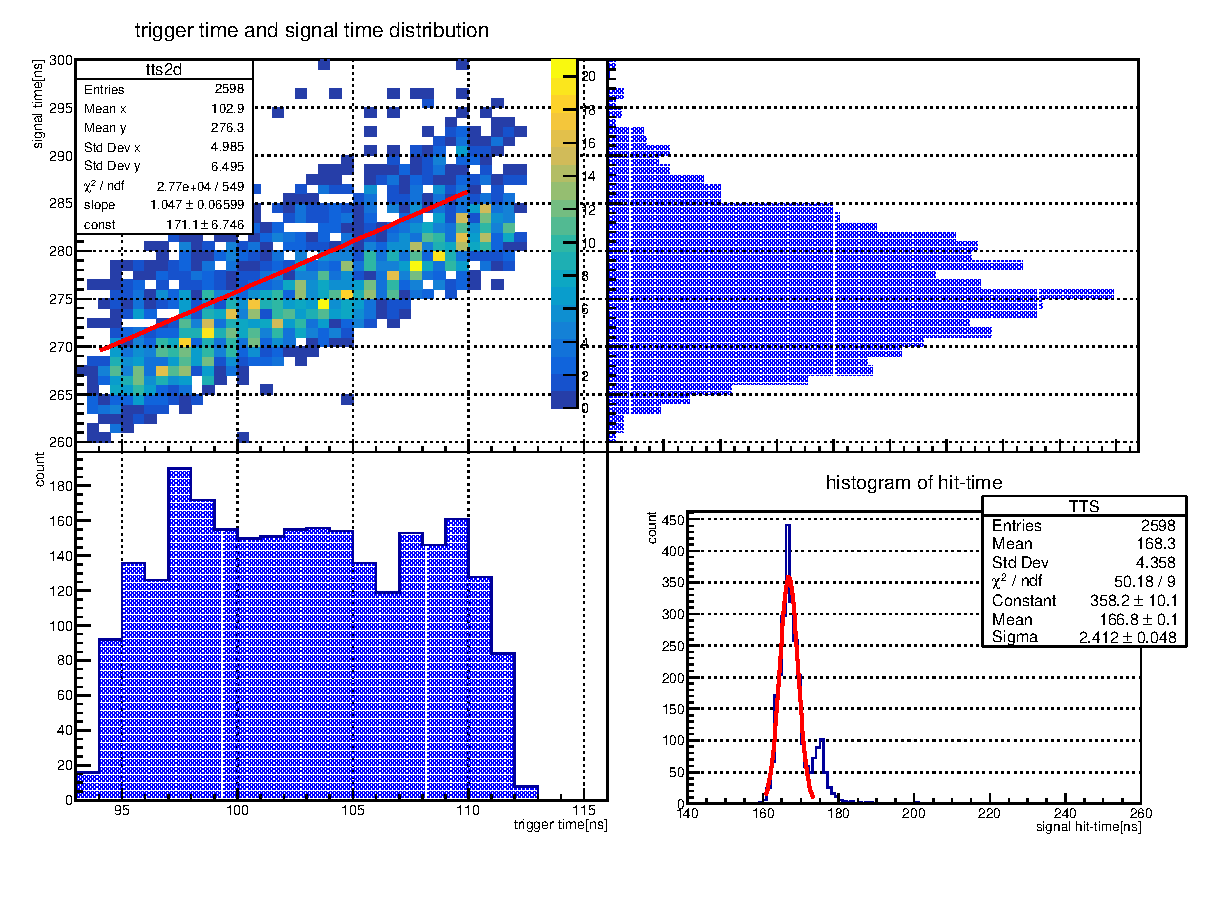
\includegraphics[width=0.78\textwidth]{typical_hittime} % 单图
%\end{figure}
\end{frame}
%%%%%%%%%%%%%%%%%%%%%%%%%%%%%%%%%%%%%%%%%%%
\begin{frame}{requirements}
\begin{enumerate}
\item sotre the raw waveform data(.1pe, 1pe, TTS).
\item store the auxilary testing information(container #, mass#, HV, DCR. etc).
\item easy to manage (create, modify and update) and analyze.
\item \alert{one ane acquire almost all the data needed for analysis(of one PMT) from only one file.}
\end{enumerate}
\end{frame}
%%%%%%%%%%%%%%%%%%%%%%%%%%%%%%%%%%%%%%%%%%%
\begin{frame}{prliminary structure}
\begin{itemize}
\item each PMT have one root file named in "SN\_rawdata.root"
\item In a specific root file, we have several trees and a auxilary data class
\end{itemize}

\end{frame}
%%%%%%%%%%%%%%%%%%%%%%%%%%%%%%%%%%%%%%%%%%%
\begin{frame}{PMT testing report-pass}
We have generated testing report for each qualified PMT.
\vspace{-.2cm}
\begin{figure}
\centering
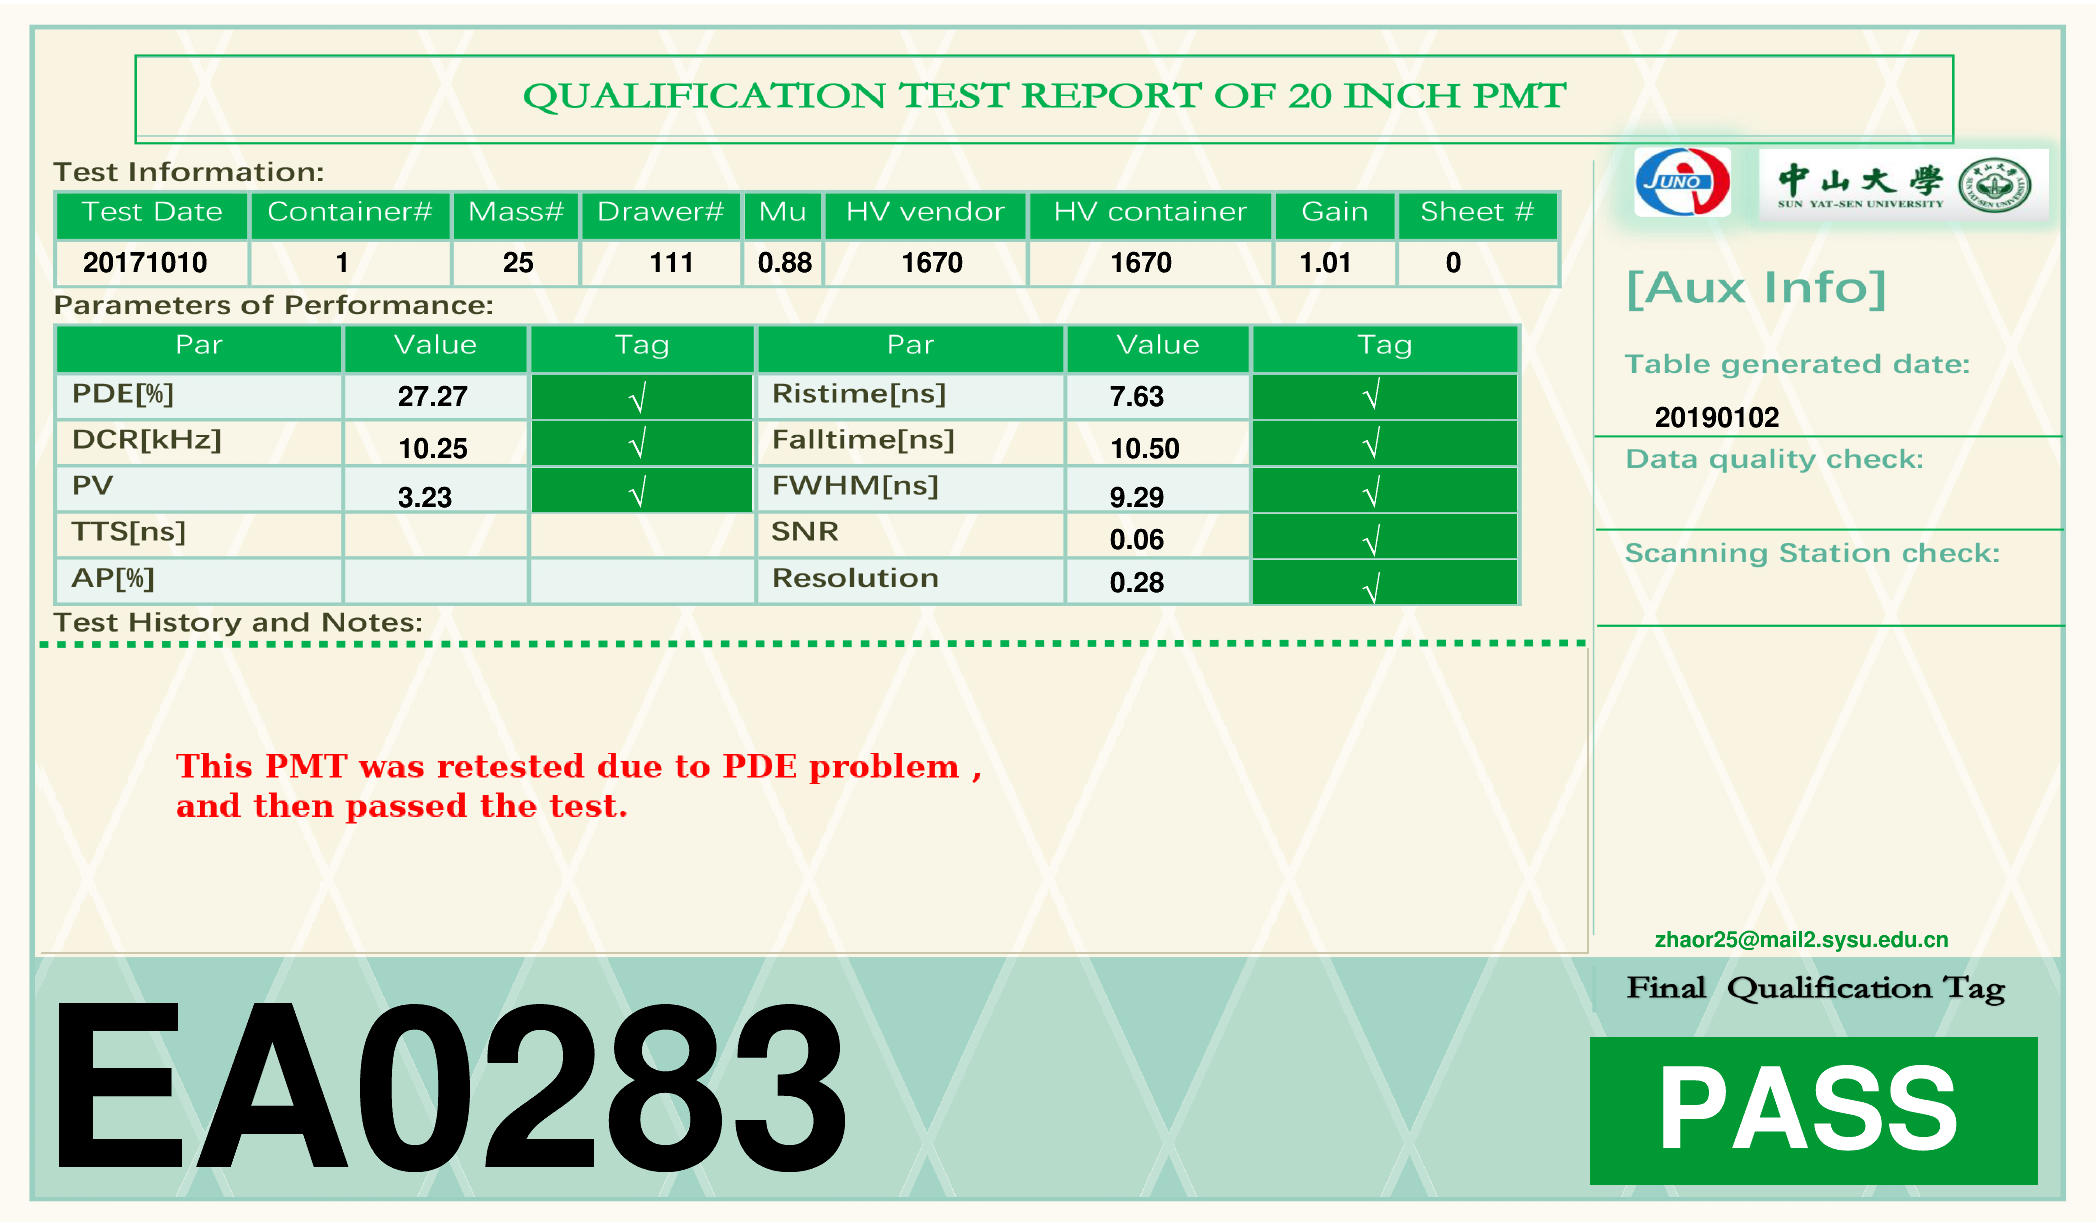
\includegraphics[width=1.0\textwidth]{figures/SN_EA0283_pde1_dcr1_HV1_pv1_rt1_tag1.png}
\end{figure}
\end{frame}
%%%%%%%%%%%%%%%%%%%%%%%%%%%%%%%%%%%%%%%%%%%
%\begin{frame}{calibration of each drawer}
%Generally, we put several PMTs with known PDE value\footnote{or QE value}  into one drawer and linearly fit the PDE-$\mu_{test}$ data to get \alert{drawer$_{factor}$}.
%\vspace{.5cm}
%\hrule{\textwidth}
%\vspace{.5cm}
%
%While an alternative way to access the drawer$_{factor}$ is fitting PDE-$\mu_{test}$ data {\color{red}from all the PMTs tested in one drawer rather than the mannual selected ones.} Then once we finish one PMT test in a drawer we will get one more statistical sample in the PDE-$\mu_{test}$ fitting, and we could expect that the fitted drawer$_{factor}$ will get more stable as we testing more PMTs.
%
%\vspace{.5cm}
%The advantage of this "self-calibration" method is that we could {\color{red}decrease the statistical error as much as possible}; and the remained fluctuation of drawer$_{factor}$ can be the system error.
%\end{frame}
\section{Waveform and Charge Spectrum}
%%%%%%%%%%%%%%%%%%%%%%%%%%%%%%%%%%%%%%%%%%%
%\begin{frame}{抽屉刻度方法}
%滨松厂家提供部分PMT的QE\footnote{假定所有的PMT的收集效率相同}值,可以从PMT数据库\footnote{王俊[http://pmtdb.juno.ihep.ac.cn/index.html]}查询到。如果某一个抽屉测到的滨松PMT恰好有QE的厂家值,就选用它进行刻度。
%
%\vspace{.5cm}
%\hrule{\textwidth}
%\vspace{.5cm}
%为了保证刻度PMT的性能,只选取通过集装箱测试的PMT进行刻度。
%\end{frame}
%%%%%%%%%%%%%%%%%%%%%%%%%%%%%%%%%%%%%%%%%%%
%\begin{frame}{一个抽屉的刻度结果}
%随着测试PMT数量的增加,拟合统计误差逐渐减小,$drawer_{factor}$的拟合结果趋于稳定(更多抽屉拟合结果见back-up部分)。
%\begin{figure}
%\centering
%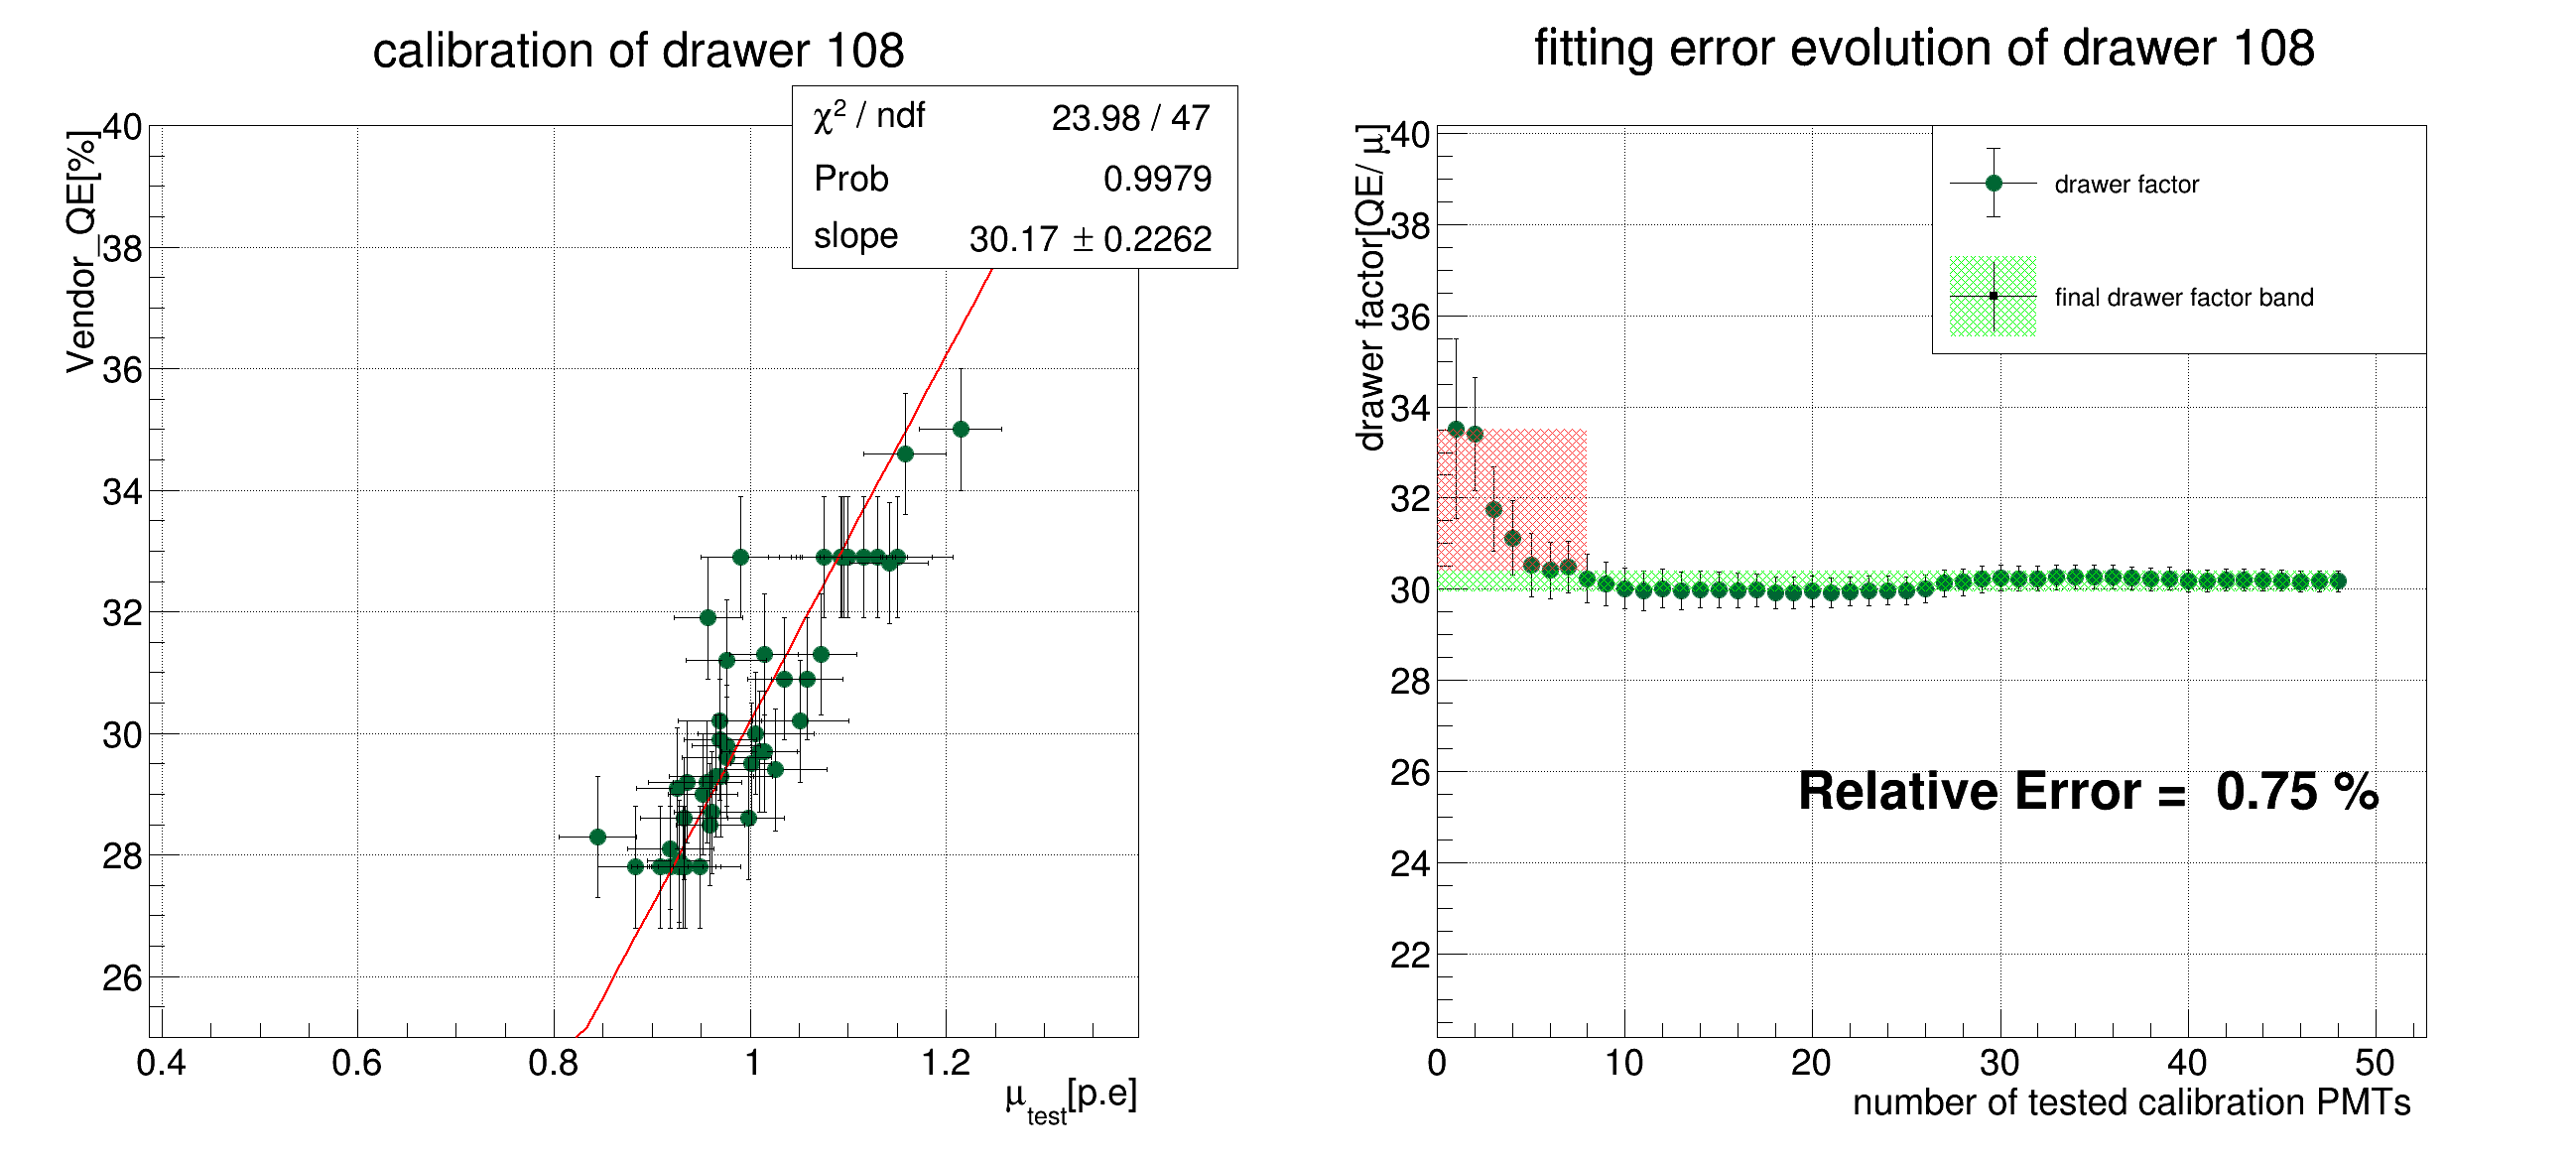
\includegraphics[width=0.98\textwidth]{sta101-7} % 单图
%\caption{108抽屉的$drawer_{factor}$拟合结果}
%\end{figure}
%\end{frame}
%%%%%%%%%%%%%%%%%%%%%%%%%%%%%%%%%%%%%%%%%%%
\begin{frame}{Typical waveform of PMT(@$gain=10^7$)}
Typical signal waveform when working @$gain=10^7$
\begin{columns}
\begin{column}{.485\textwidth}
\begin{figure}
\centering
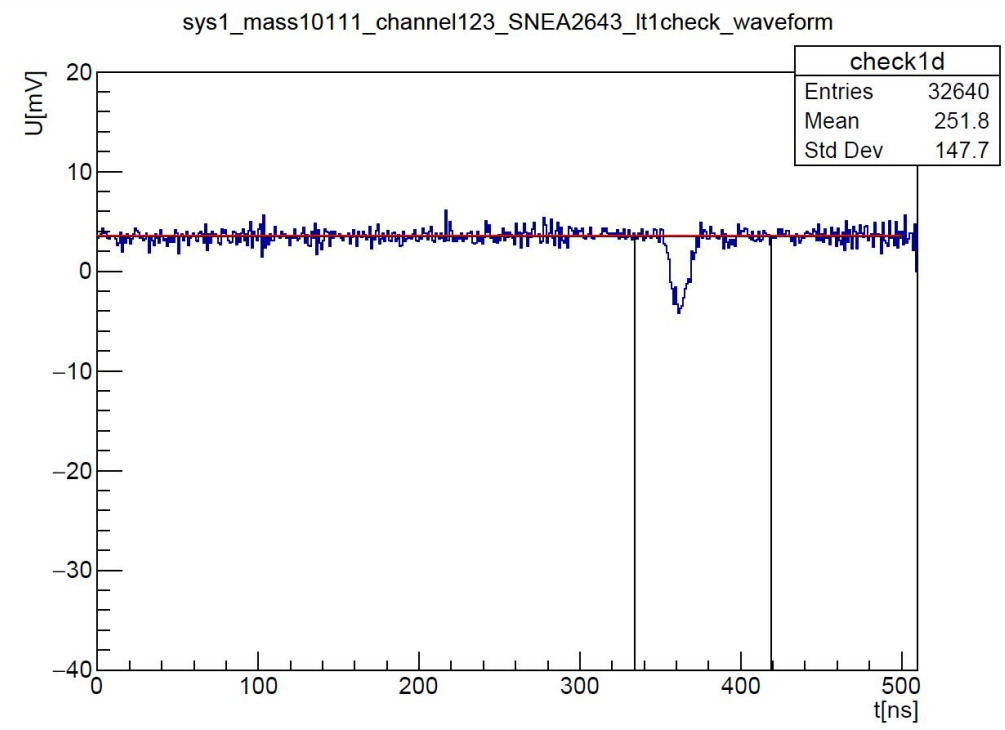
\includegraphics[width=\textwidth]{figures/hamwave.png} % 单图
%\label{fig:wave2d}
\caption{single photon signal waveform of HAMAMATSU PMT}
\end{figure}
\end{column}
\begin{column}{.5\textwidth}
\begin{figure}
\centering
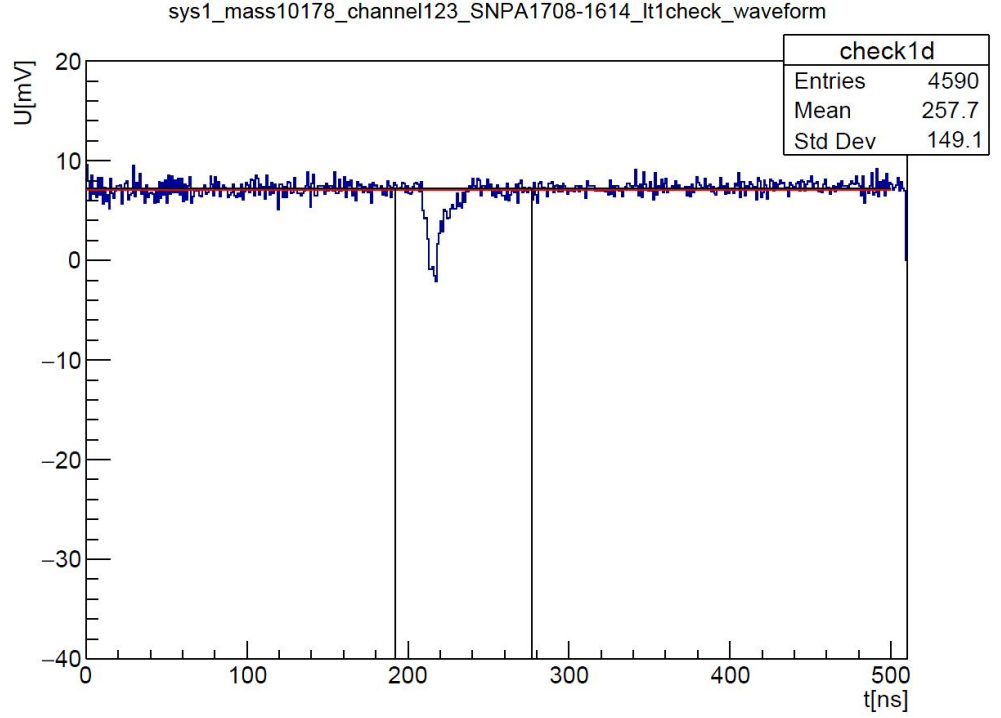
\includegraphics[width=\textwidth]{figures/mcpwave.png} % 单图
%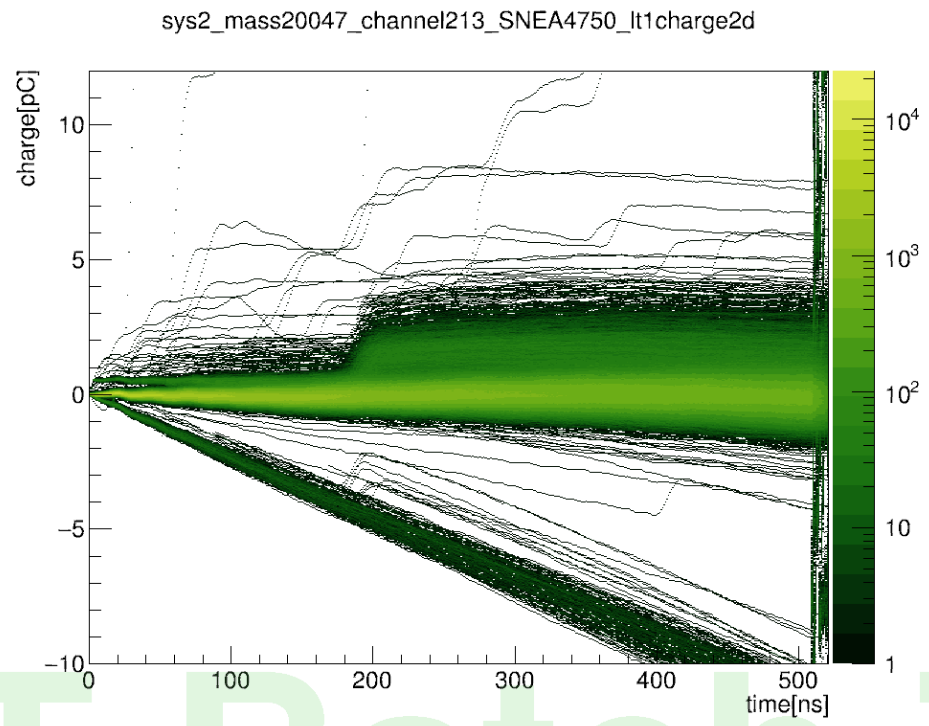
\includegraphics[width=\textwidth]{figures/baseline2d.png} % 单图
\caption{single photon signal waveform of NNVT PMT}
\end{figure}
\end{column}
\end{columns}
\end{frame}
%%%%%%%%%%%%%%%%%%%%%%%%%%%%%%%%%%%%%%%%%%%
%~~!!!!!!!!!!!!!!!!!!put two figures to illustrate!!!!!
\begin{frame}{Output waveforms of PMT @$Gain=10^7$}
The 2-D waveform histogram contains all the recorded waveforms, we can clearly see the "delayed signals" of HAMMATSU PMT and "big signals" of NNVT PMTs.
\begin{columns}
\begin{column}{.47\textwidth}
\begin{figure}
\centering
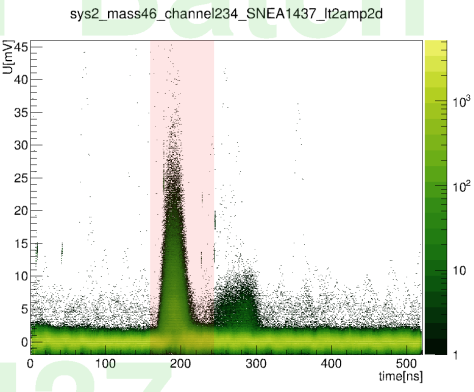
\includegraphics[width=\textwidth]{figures/wave2d.png} % 单图
%\label{fig:wave2d}
\caption{all frames of HAMAMATSU PMT}
\end{figure}
\end{column}
\begin{column}{.5\textwidth}
\begin{figure}
\centering
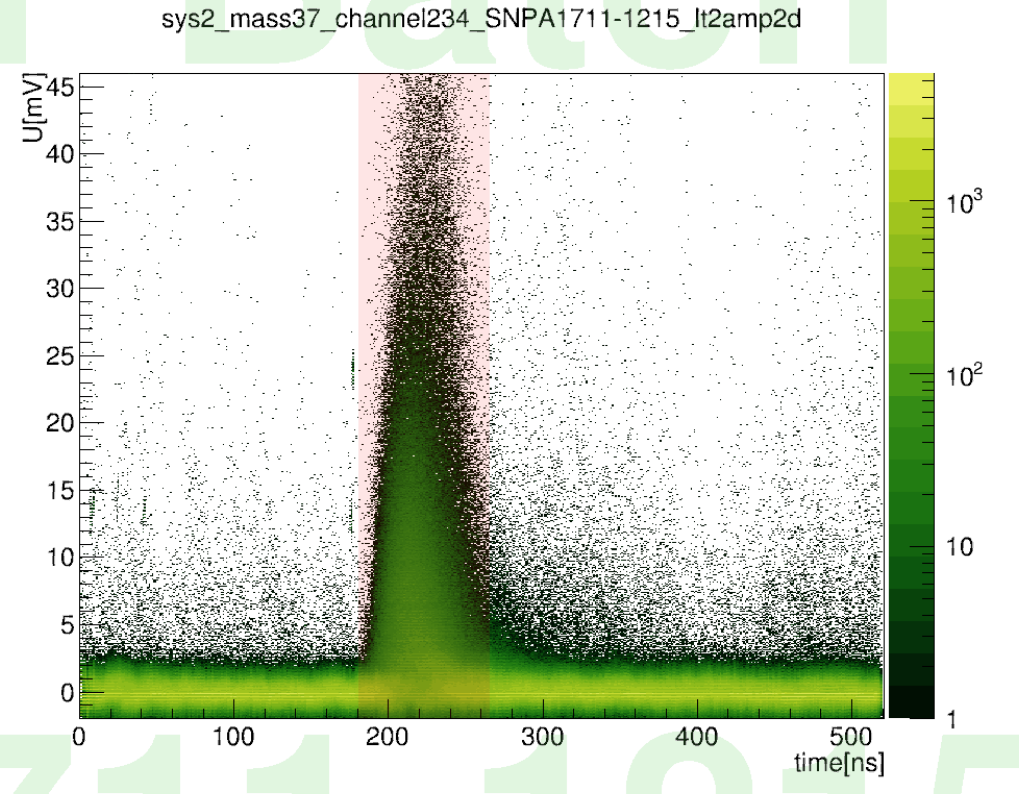
\includegraphics[width=\textwidth]{figures/mcpwave2d.png} % 单图
%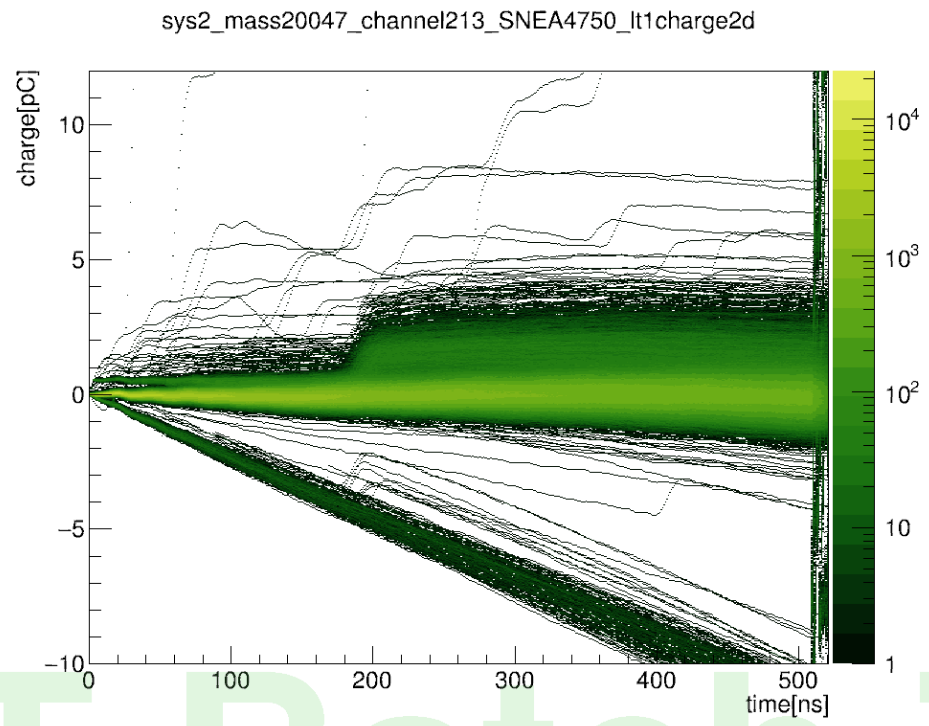
\includegraphics[width=\textwidth]{figures/baseline2d.png} % 单图
\caption{all frames of NNVT PMT}
\end{figure}
\end{column}
\end{columns}
\end{frame}
%%%%%%%%%%%%%%%%%%%%%%%%%%%%%%%%%%%%%%%%%%%
\begin{frame}{Output integrated waveforms of PMT(@$gain=10^7$)}
From the waveform integral histogram we acquire more information.
\begin{columns}
\begin{column}{.5\textwidth}
\begin{figure}
\centering
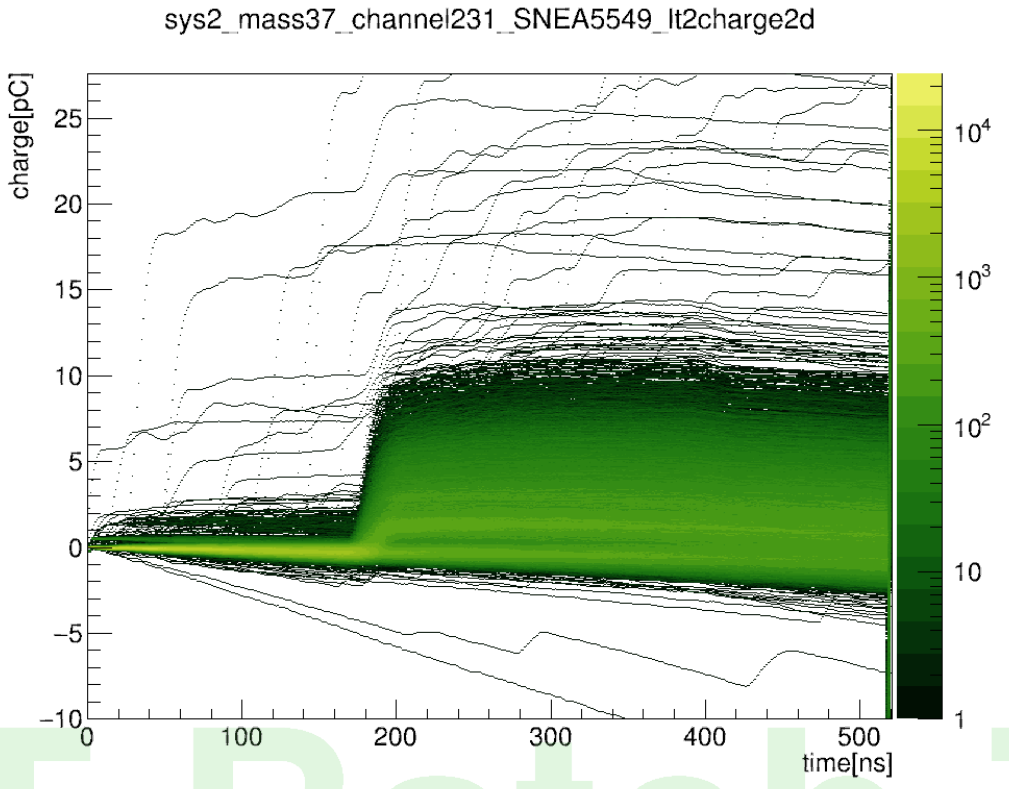
\includegraphics[width=\textwidth]{figures/hambaseline2d.png} % 单图
%\label{fig:wave2d}
\caption{integrated waveforms of HAMAMATSU PMT}
\end{figure}
\end{column}
\begin{column}{.5\textwidth}
\begin{figure}
\centering
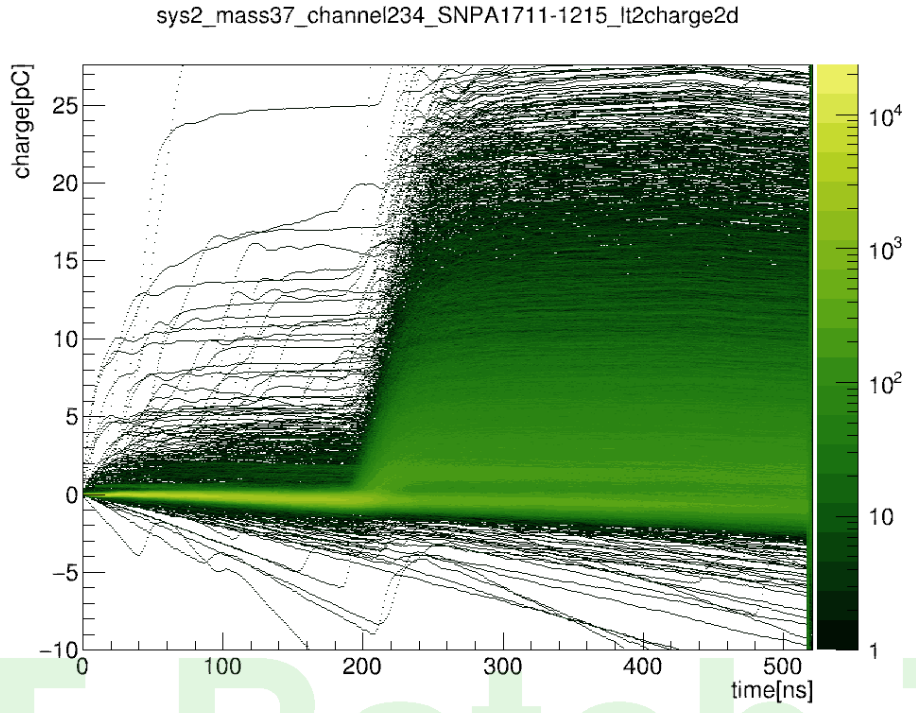
\includegraphics[width=\textwidth]{figures/mcpbaseline2d.png} % 单图
%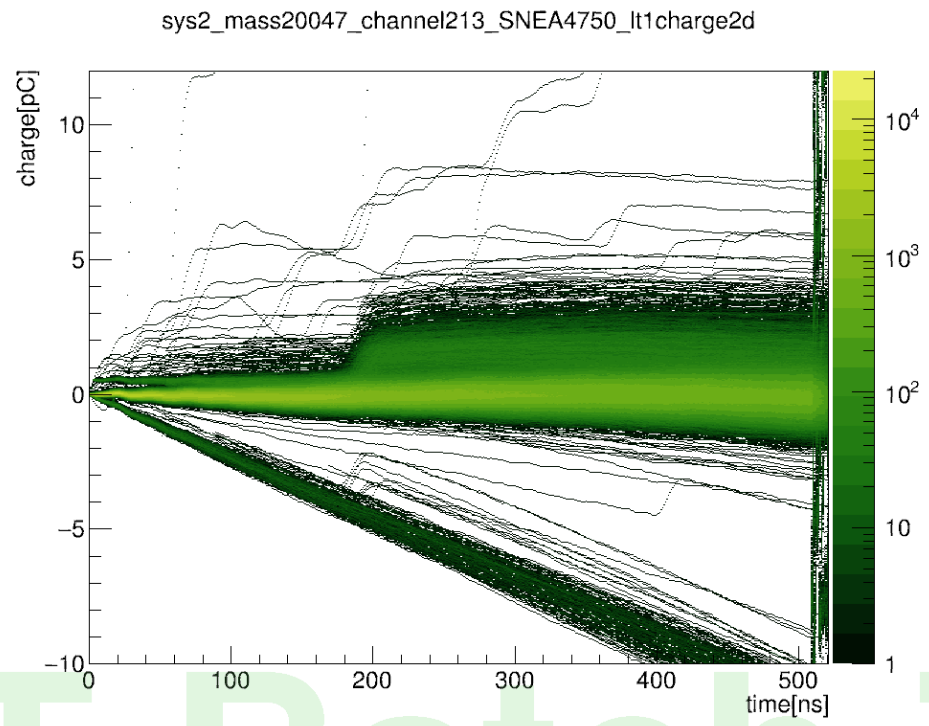
\includegraphics[width=\textwidth]{figures/baseline2d.png} % 单图
\caption{integrated waveforms of NNVT PMT}
\end{figure}
\end{column}
\end{columns}
\end{frame}
%%%%%%%%%%%%%%%%%%%%%%%%%%%%%%%%%%%%%%%%%%%
\begin{frame}{Amplitude spectrum (@$gain=10^7\&\&\mu\simeq 1.3$)}
Signal amplitude stability of NNVT PMT is worse than HAMAMATSU PMT.
\vspace{-.3cm}
\begin{columns}
\begin{column}{.5\textwidth}
\begin{figure}
\centering
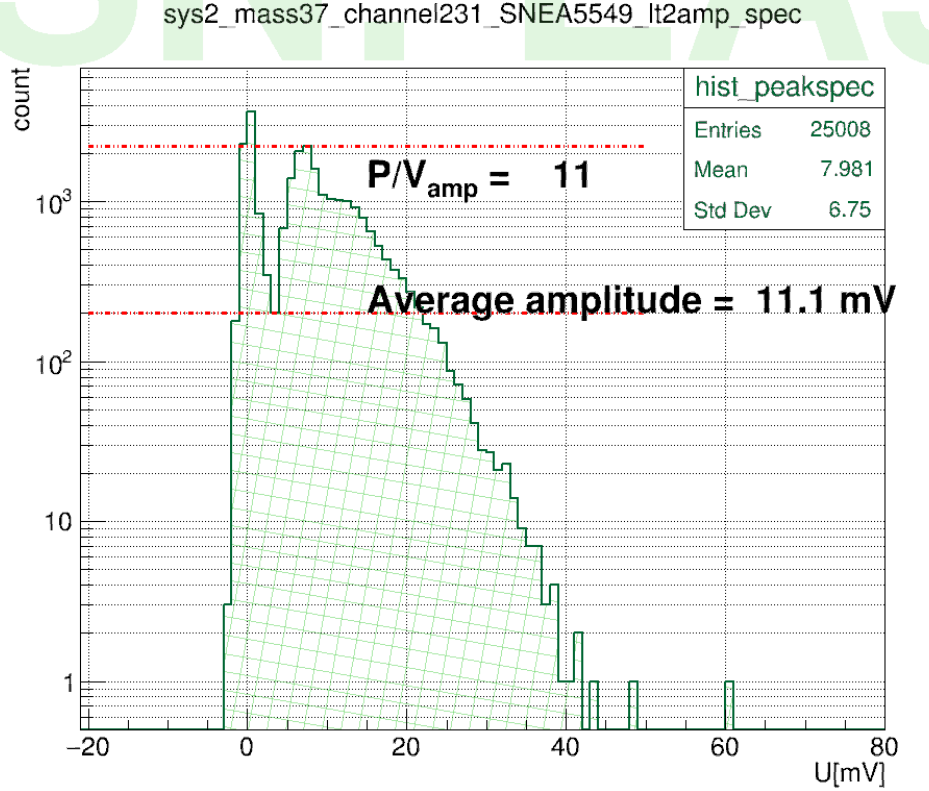
\includegraphics[width=\textwidth]{figures/hamampspe.png} % 单图
%\label{fig:wave2d}
\caption{Amplitude spectrum of HAMAMATSU PMT}
\end{figure}
\end{column}
\begin{column}{.5\textwidth}
\begin{figure}
\centering
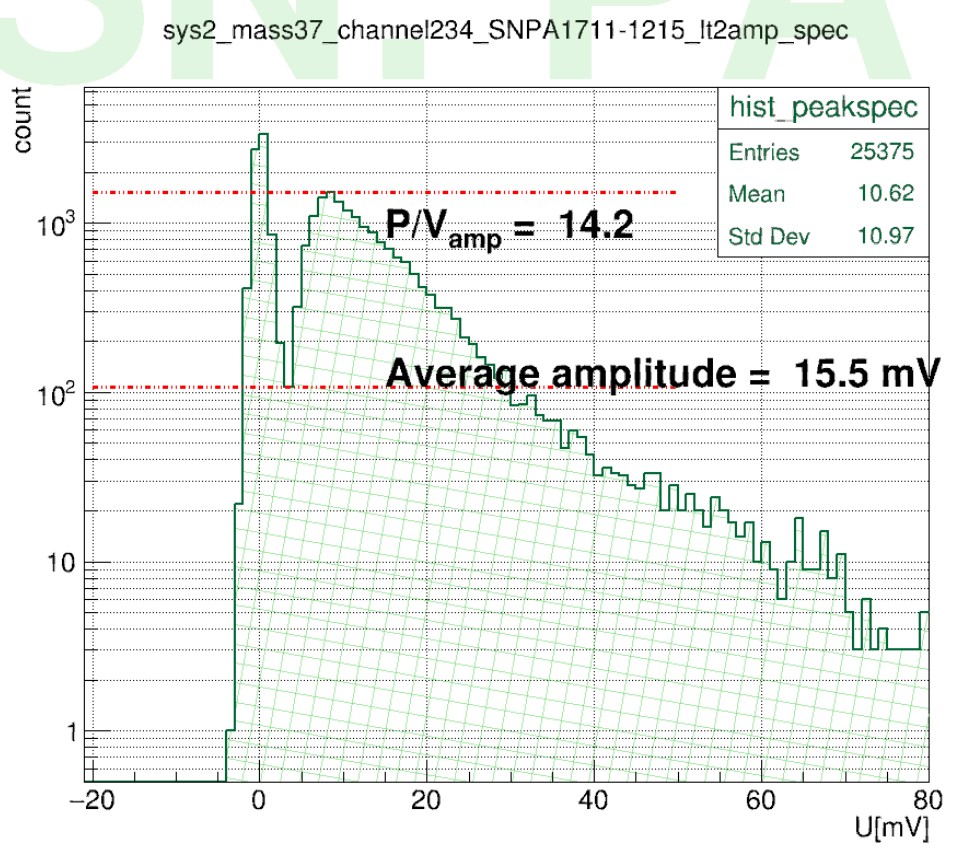
\includegraphics[width=\textwidth]{figures/mcpampspe.png} % 单图
%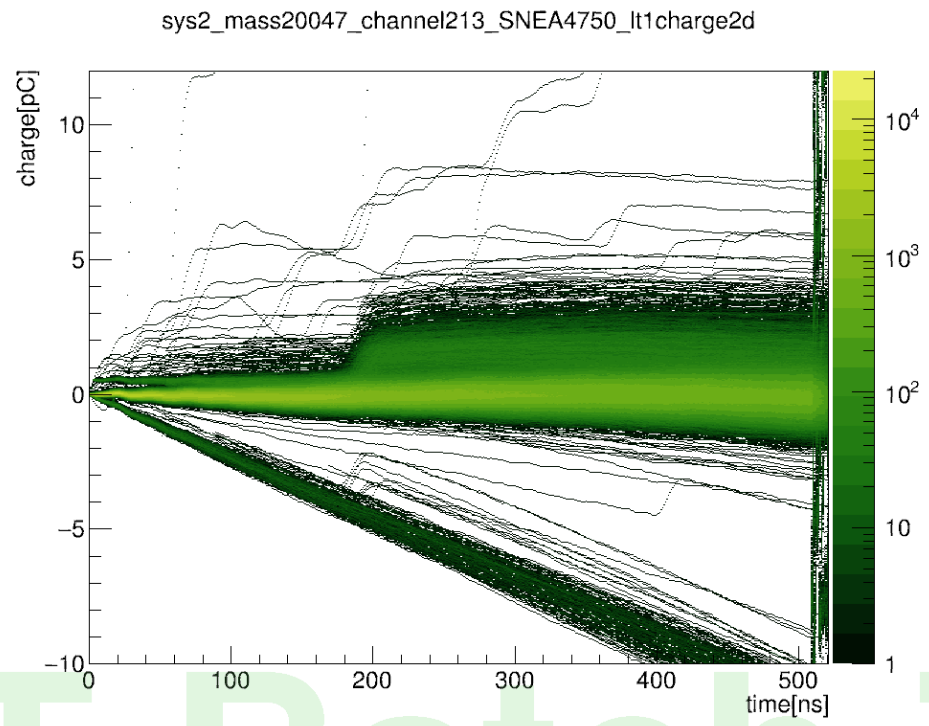
\includegraphics[width=\textwidth]{figures/baseline2d.png} % 单图
\caption{Amplitude spectrum of NNVT PMT}
\end{figure}
\end{column}
\end{columns}
\end{frame}
%%%%%%%%%%%%%%%%%%%%%%%%%%%%%%%%%%%%%%%%%%%
\begin{frame}{Aligned waveforms (@$gain=10^7\&\&\mu\simeq 1.3$)}
Aligning all signals according to their maximum: signal profile of HAMAMATSU PMT have better symetry.
%\vspace{-.3cm}
\begin{columns}
\begin{column}{.5\textwidth}
\begin{figure}
\centering
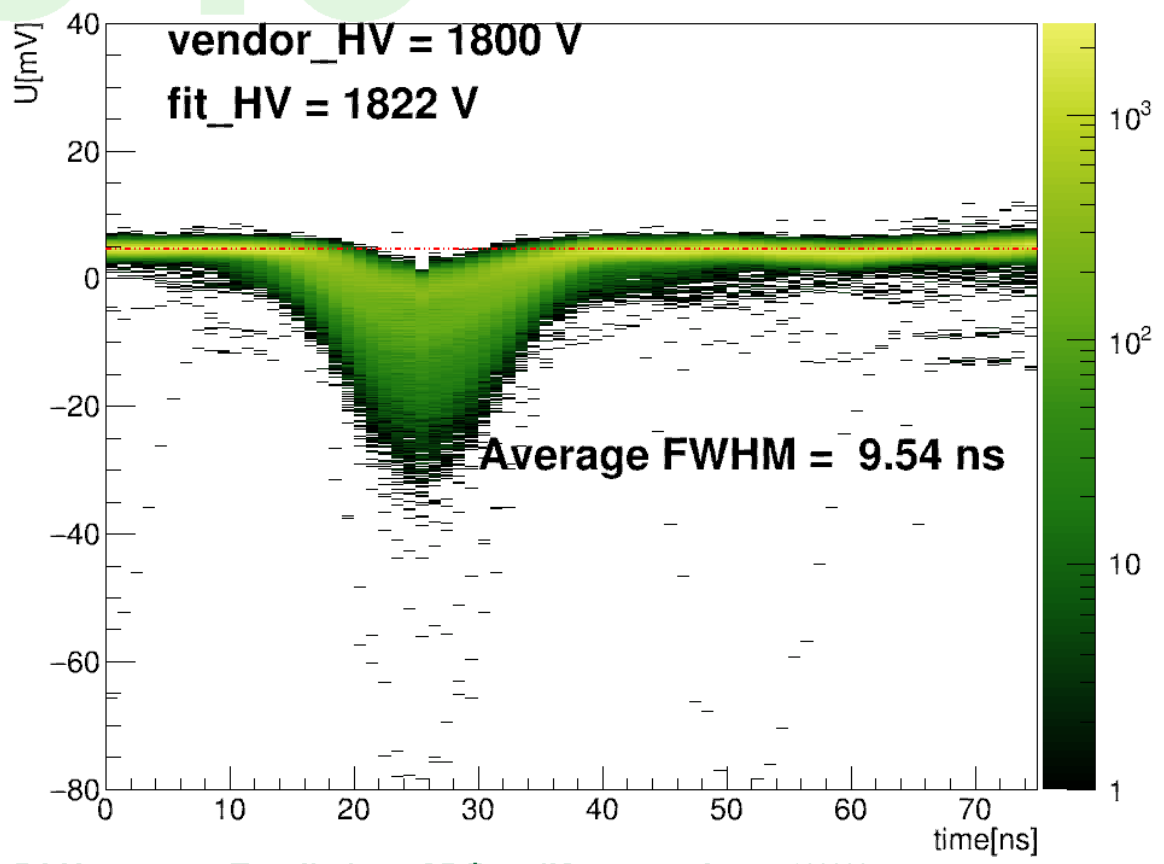
\includegraphics[width=\textwidth]{figures/hamaligned2d.png} % 单图
%\label{fig:wave2d}
\caption{Aligned frames of HAMAMATSU PMT}
\end{figure}
\end{column}
\begin{column}{.5\textwidth}
\begin{figure}
\centering
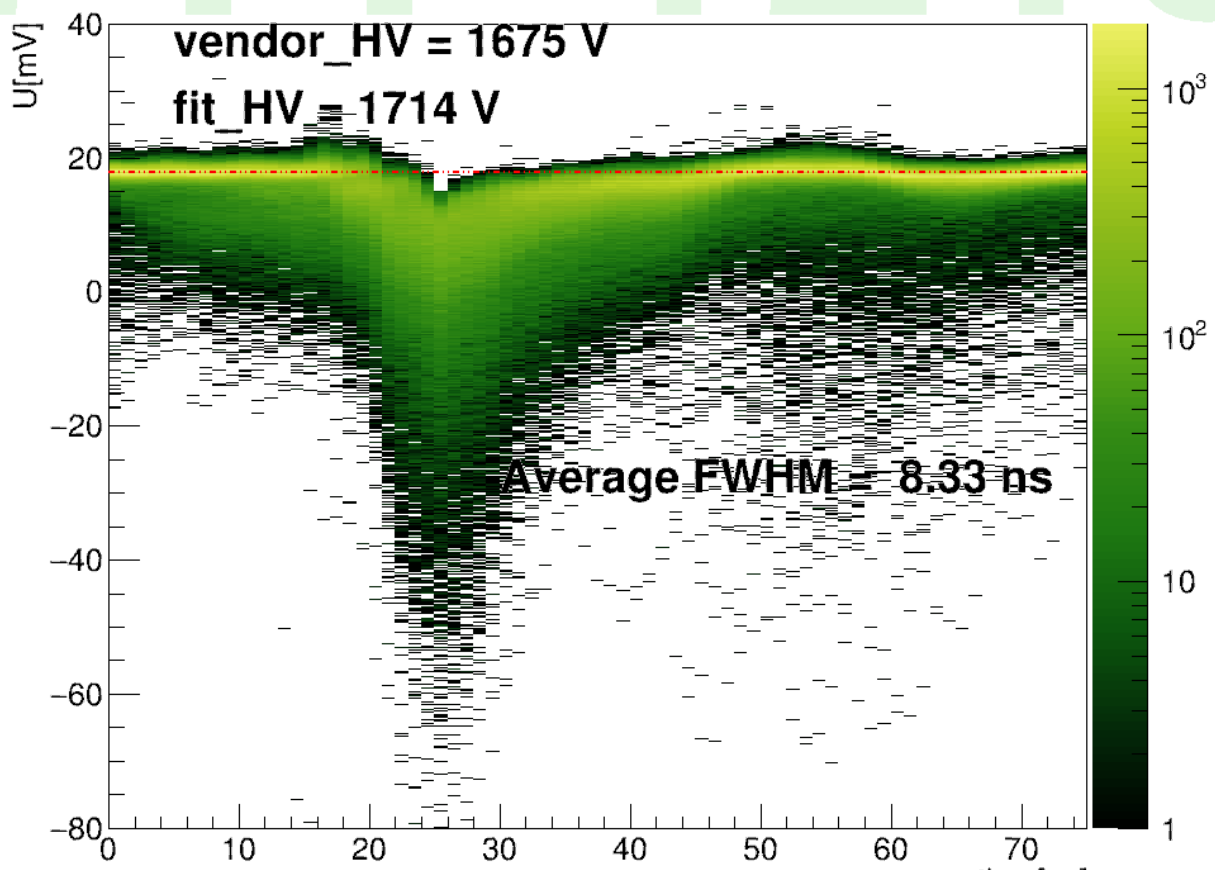
\includegraphics[width=\textwidth]{figures/mcpaligned2d.png} % 单图
%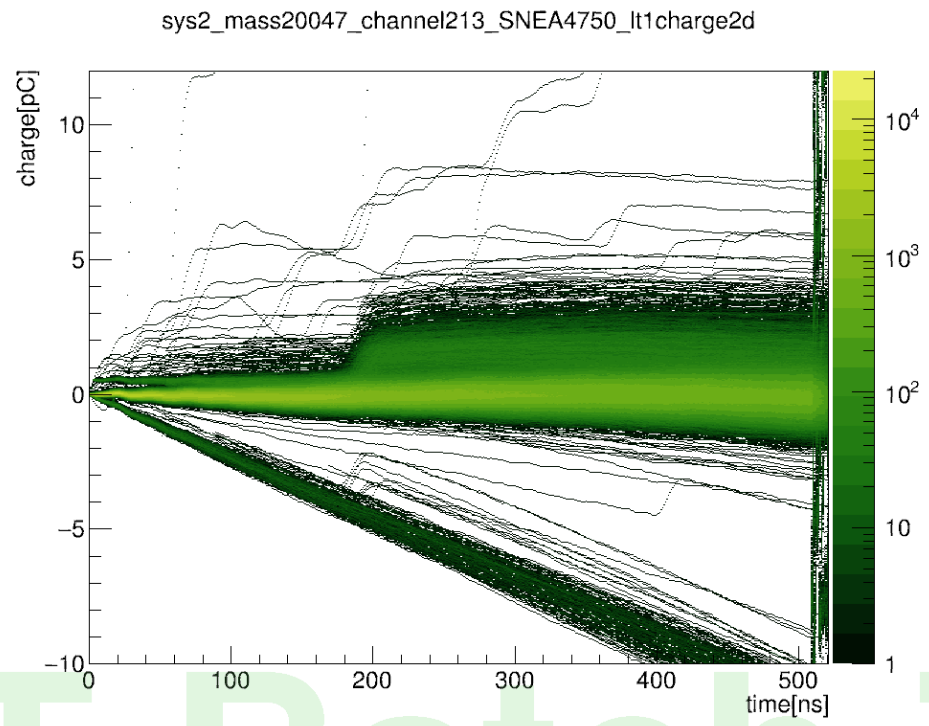
\includegraphics[width=\textwidth]{figures/baseline2d.png} % 单图
\caption{Aligned frames \ of \ NNVT \ PMT}
\end{figure}
\end{column}
\end{columns}
\end{frame}
%%%%%%%%%%%%%%%%%%%%%%%%%%%%%%%%%%%%%%%%%%%
\begin{frame}{Average waveform (@$gain=10^7\&\&\mu\simeq 1.3$)}
The average waveform of NNVT PMT has faster rising edge and lower falling edge.
\vspace{-.3cm}
\begin{columns}
\begin{column}{.5\textwidth}
\begin{figure}
\centering
%\label{fig:wave2d}
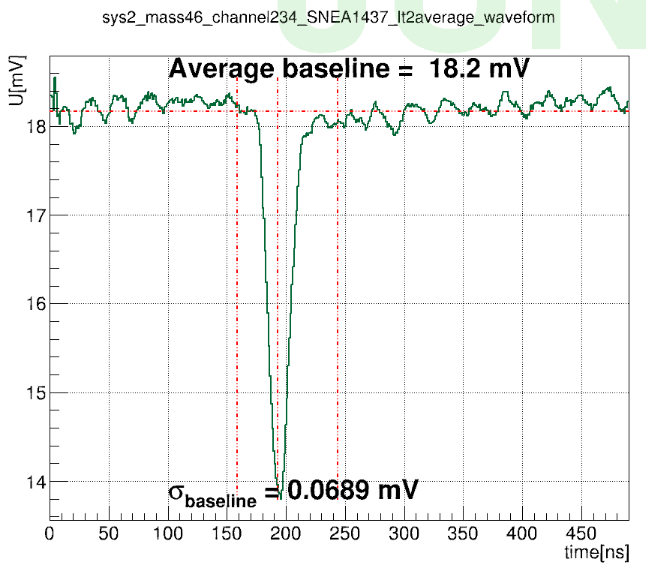
\includegraphics[width=\textwidth]{figures/avewave.png} % 单图
\caption{average waveform of HAMAMATSU PMT}
\end{figure}
\end{column}
\begin{column}{.5\textwidth}
\begin{figure}
\centering
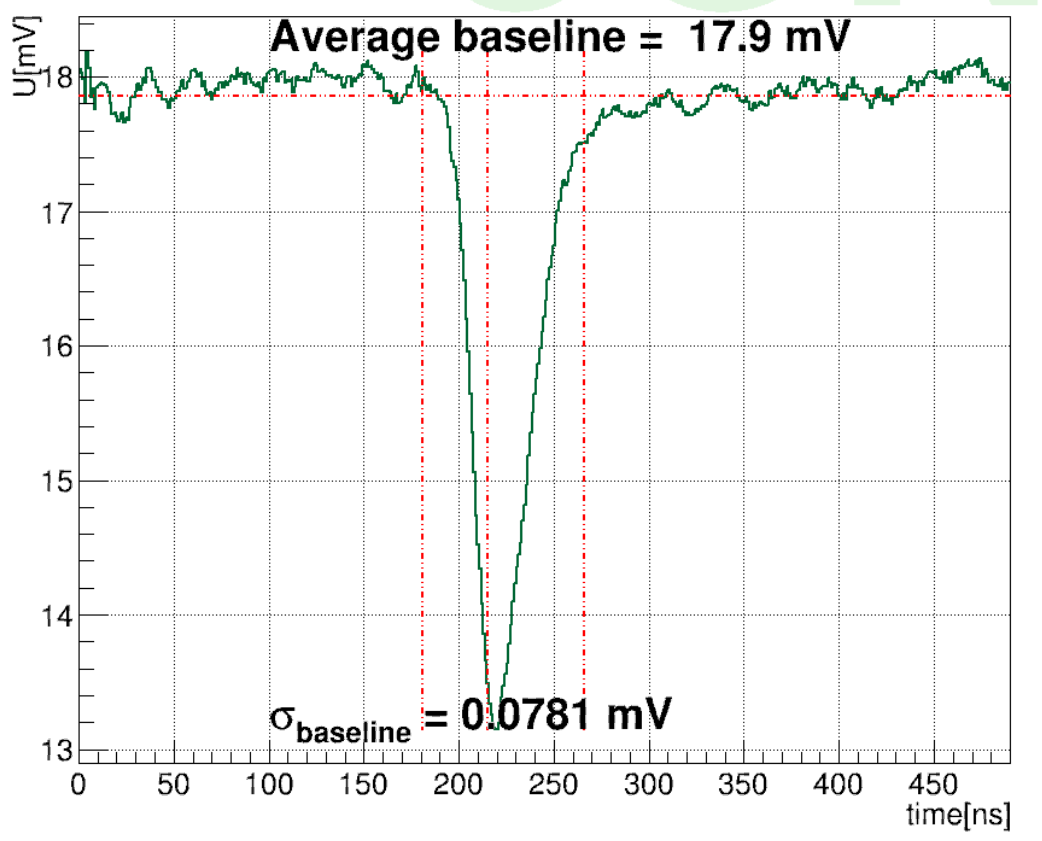
\includegraphics[width=\textwidth]{figures/mcpavewave.png} % 单图
\caption{average waveform of NNVT PMT}
\end{figure}
\end{column}
\end{columns}
\end{frame}
%\section{参数计算和结果分析}
\begin{frame}{Signal hit time distribution}
The hittime response of NNVT PMT is about 20ns slower than the HAMAMATSU PMT.
%\vspace{-.6cm}
\begin{columns}
\begin{column}{.5\textwidth}
\begin{figure}
\centering
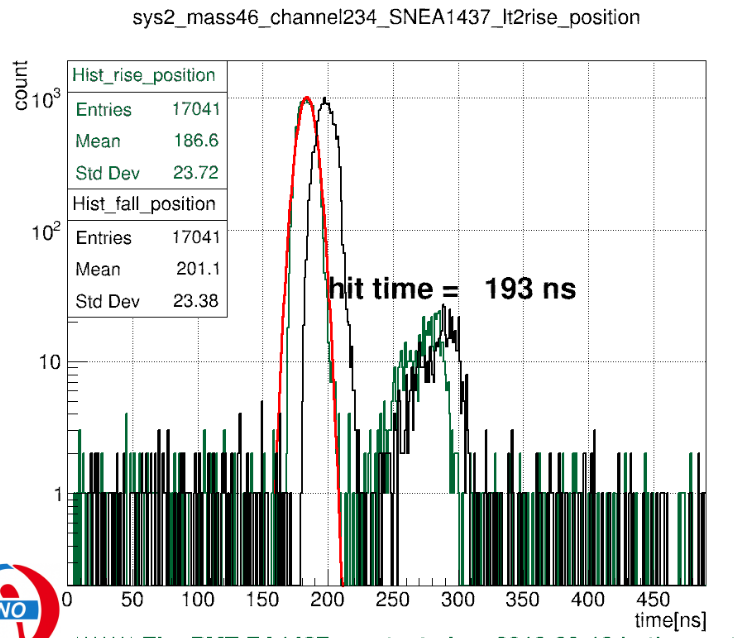
\includegraphics[width=\textwidth]{figures/riseposition.png} % 单图
%\label{fig:wave2d}
\caption{hit time of HAMAMATSU PMT}
\end{figure}
\end{column}
\begin{column}{.5\textwidth}
\begin{figure}
\centering
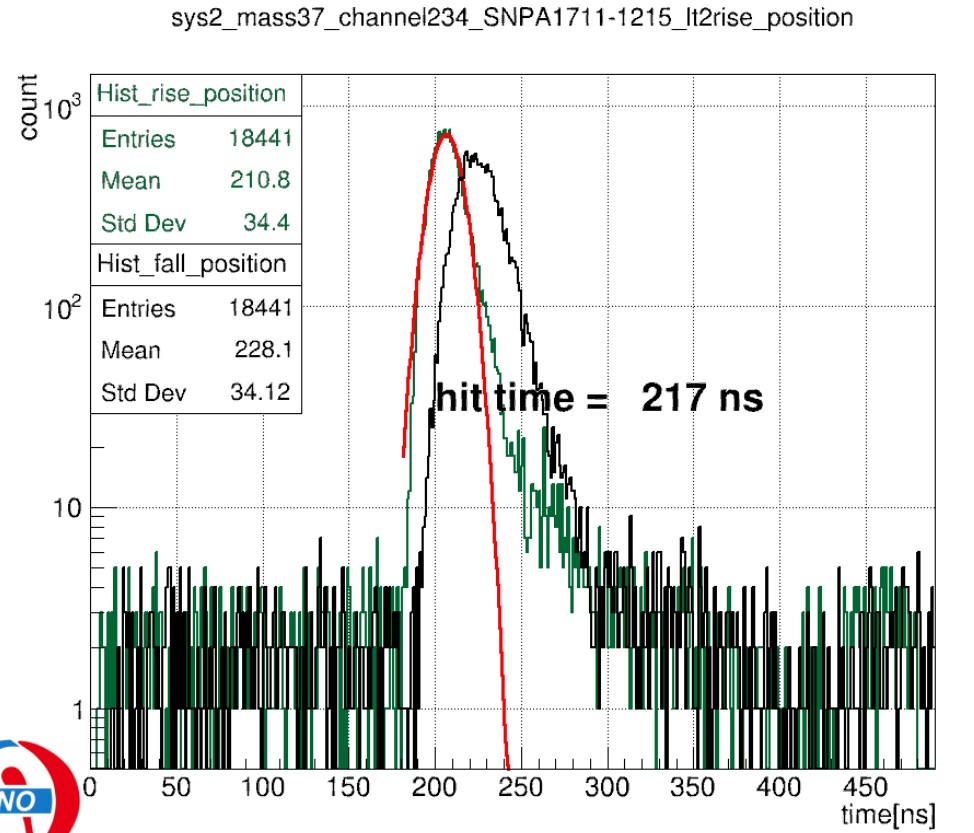
\includegraphics[width=\textwidth]{figures/hitpositionmcp.png} % 单图
\caption{hit time of NNVT PMT}
\end{figure}
\end{column}
\end{columns}
\end{frame}
%%%%%%%%%%%%%%%%%%%%%%%%%%%%%%%%%%%%%%%%%%%%%%%%%%%%%%
\begin{frame}{charge and amplitude (@$gain=10^7\&\&\mu\simeq 1.3$)}
amplitudes and  and charge intergrals of NNVT PMT is not as stable as HAMAMATSU PMT.
\begin{columns}
\begin{column}{.5\textwidth}
\begin{figure}
\centering
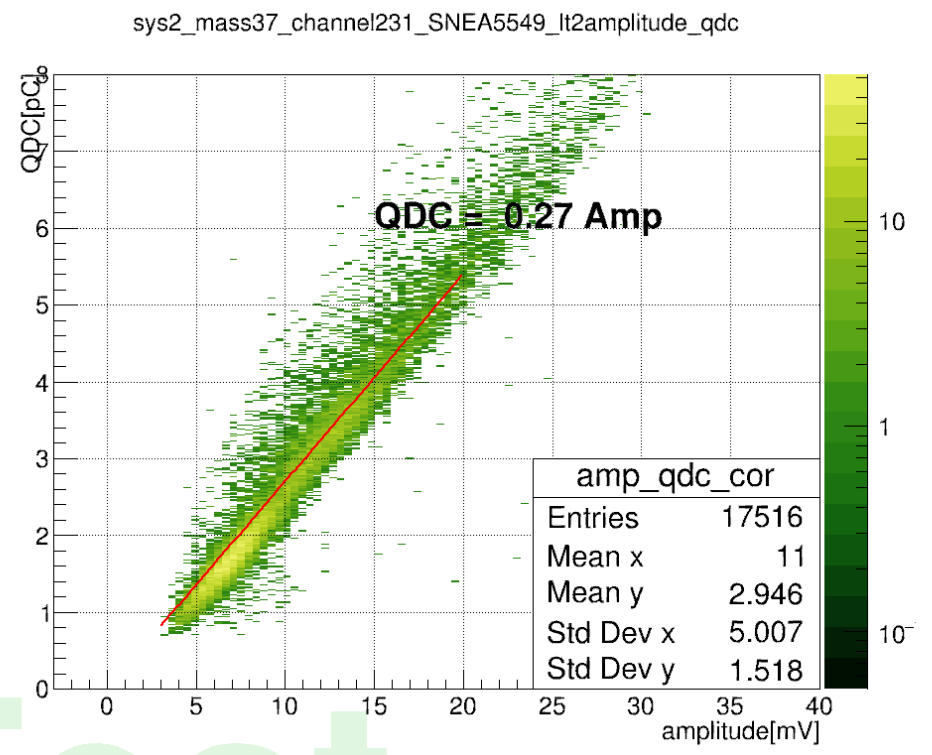
\includegraphics[width=\textwidth]{figures/hamampqdc.png} % 单图
%\label{fig:wave2d}
\caption{charge and amplitude correlation of HAMAMATSU PMT}
\end{figure}
\end{column}
\begin{column}{.5\textwidth}
\begin{figure}
\centering
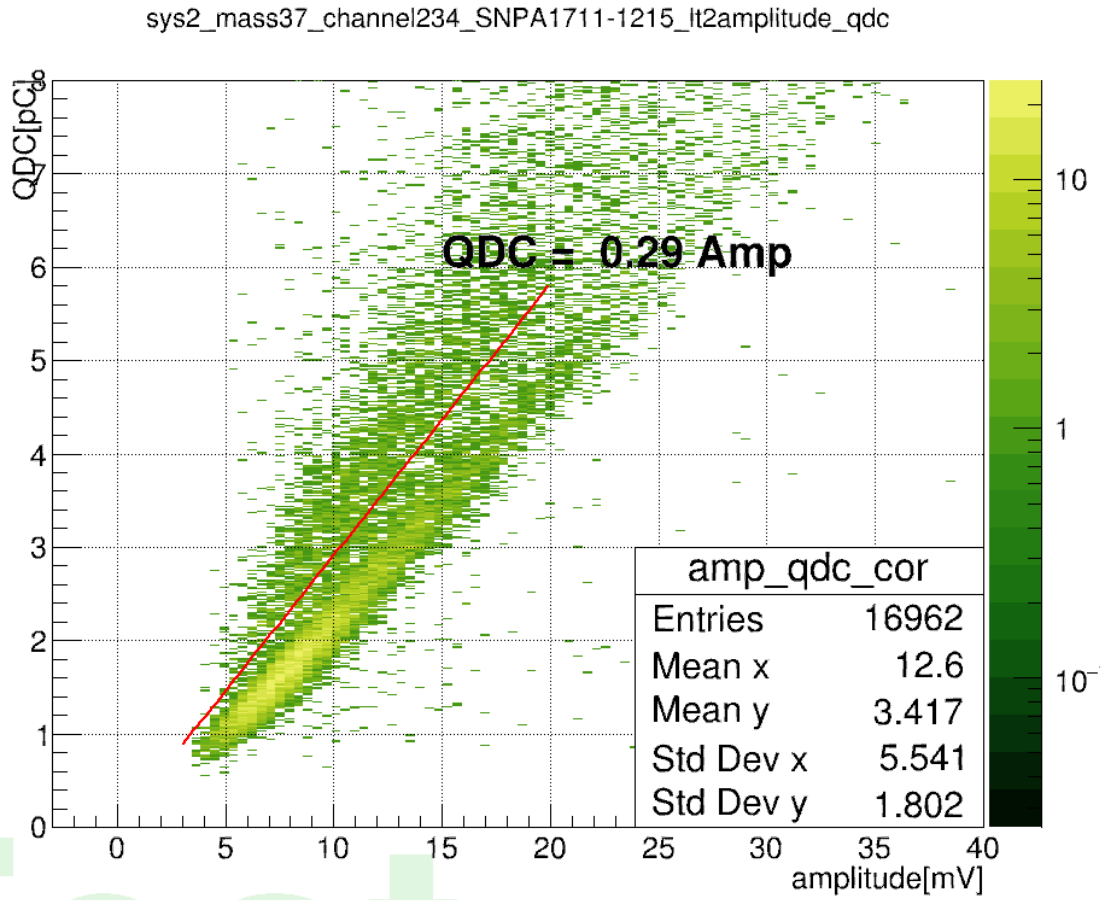
\includegraphics[width=\textwidth]{figures/mcpampqdc.png} % 单图
\caption{charge and amplitude correlation of NNVT PMT}
\end{figure}
\end{column}
\end{columns}
\end{frame}
%%%%%%%%%%%%%%%%%%%%%%%%%%%%%%%%%%%%%%%%%%%%%%%%%%%%%%
\begin{frame}{rise-time and fall-time (@$gain=10^7\&\&\mu\simeq 1.3$)}
%amplitudes and  and charge intergrals of NNVT PMT is not as stable as HAMAMATSU PMT.
\begin{columns}
\begin{column}{.5\textwidth}
\begin{figure}
\centering
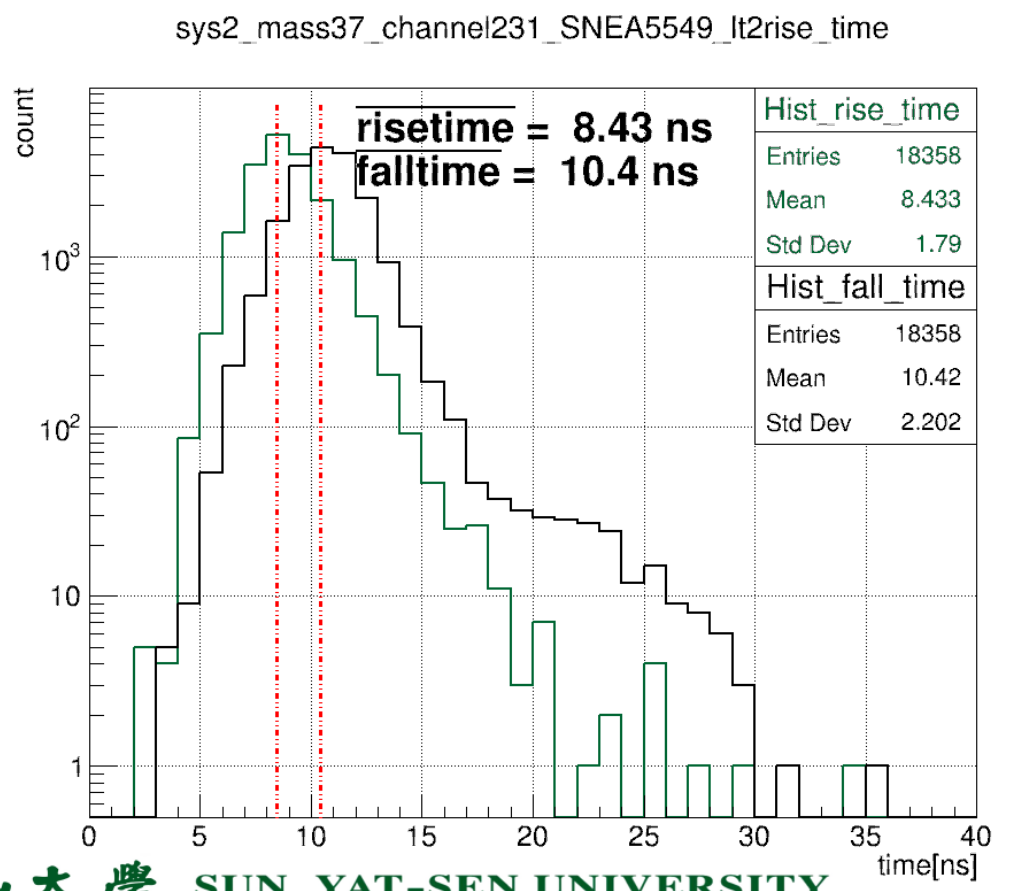
\includegraphics[width=\textwidth]{figures/hamrtft.png} % 单图
%\label{fig:wave2d}
\caption{rise-time and fall-time of HAMAMATSU PMT}
\end{figure}
\end{column}
\begin{column}{.5\textwidth}
\begin{figure}
\centering
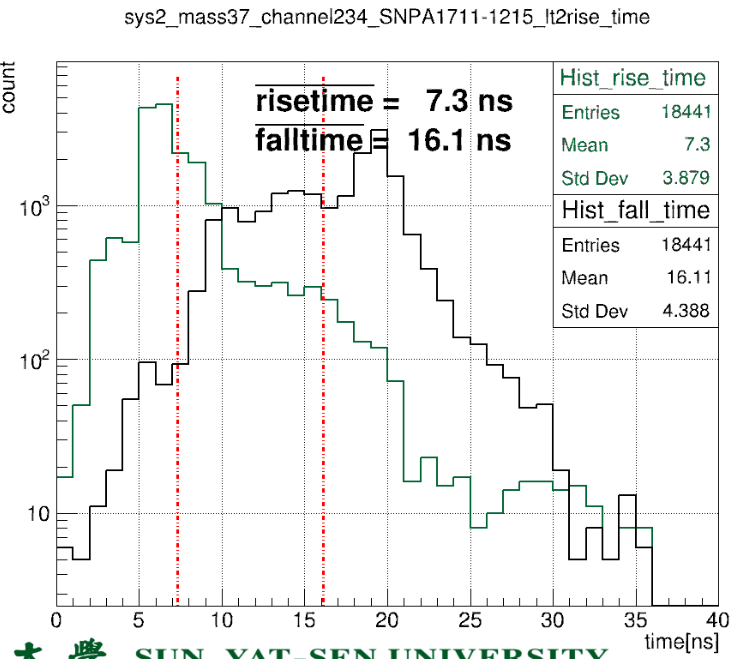
\includegraphics[width=\textwidth]{figures/mcprtft.png} % 单图
\caption{rise-time and fall-time of NNVT PMT}
\end{figure}
\end{column}
\end{columns}
\end{frame}
%%%%%%%%%%%%%%%%%%%%%%%%%%%%%%%%%%%%%%%%%%%%%%%%%%%%%%
\begin{frame}{Signal charge spectrum(@$gain=10^7\&\&\mu\simeq 1.3$)}
%amplitudes and  and charge intergrals of NNVT PMT is not as stable as HAMAMATSU PMT.
\begin{columns}
\begin{column}{.5\textwidth}
\begin{figure}
\centering
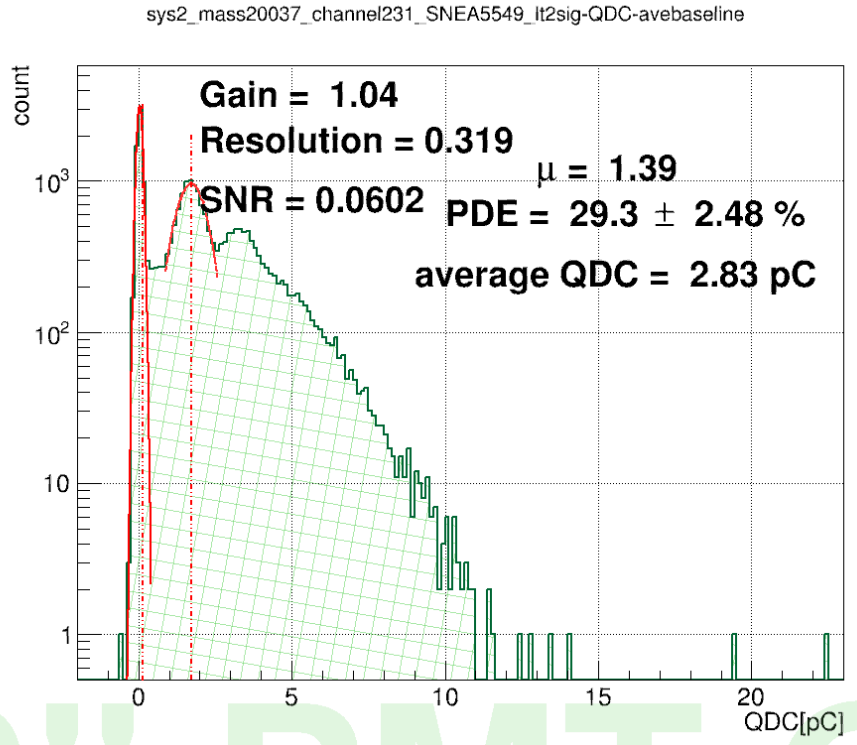
\includegraphics[width=\textwidth]{figures/hamcharge.png} % 单图
%\label{fig:wave2d}
\caption{signal charge spectrum of HAMAMATSU PMT}
\end{figure}
\end{column}
\begin{column}{.5\textwidth}
\begin{figure}
\centering
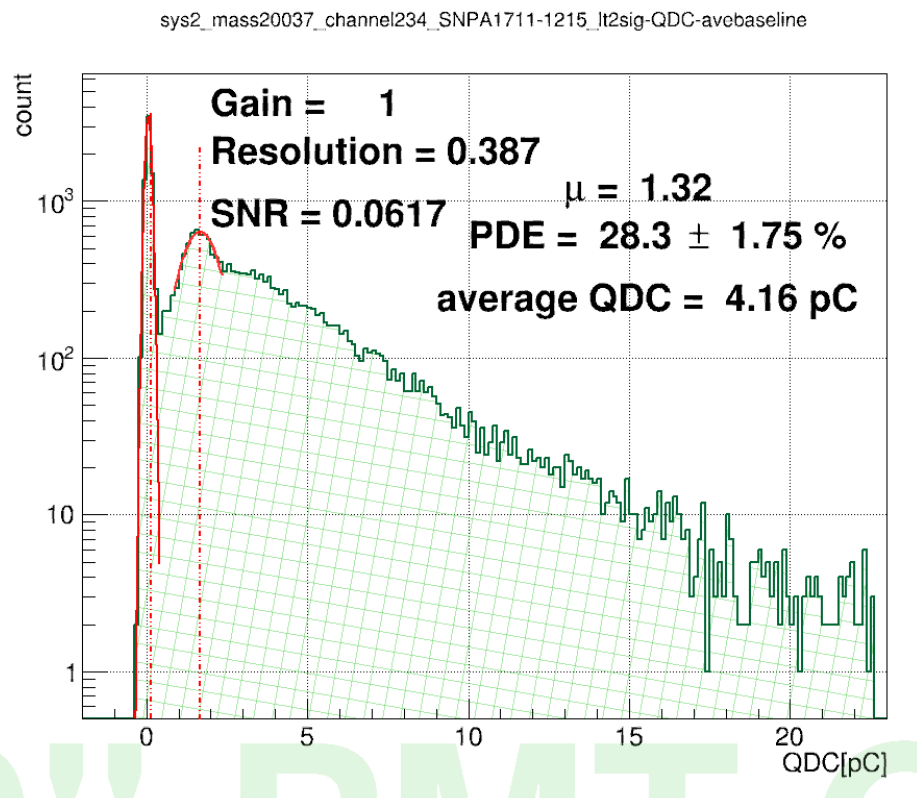
\includegraphics[width=\textwidth]{figures/mcpcharge.png} % 单图
\caption{rise-time and fall-time of NNVT PMT}
\end{figure}
\end{column}
\end{columns}
\end{frame}
%~~!!!!!!!!!!!!!!!!!!put two figures to illustrate!!!!!
%\begin{frame}{抽屉刻度结果分析\footnote{拟合出的抽屉因子与现场所使用的抽屉因子的关联见back-up部分}}
%\begin{columns}
%\begin{column}{.5\textwidth}
%\begin{figure}
%\centering
%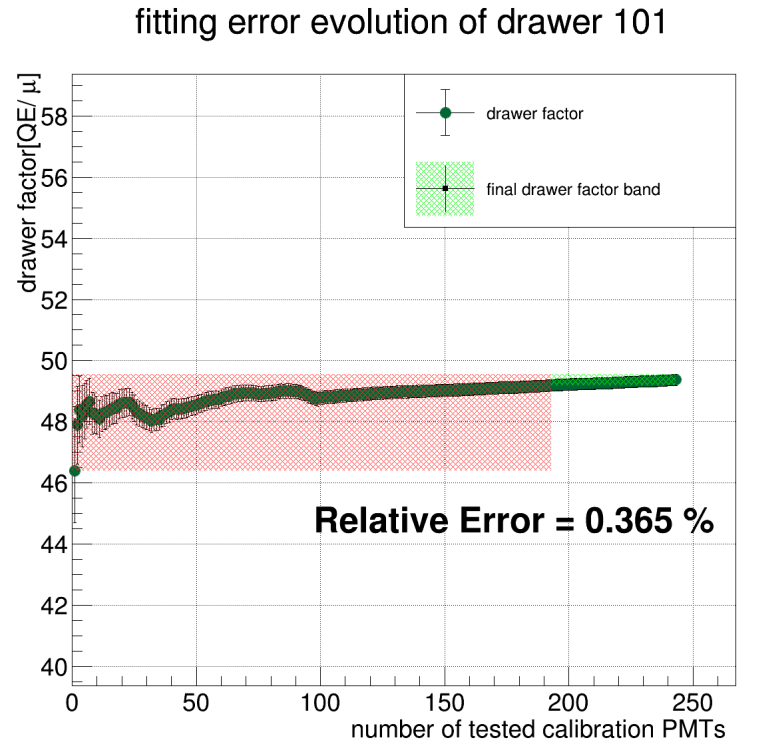
\includegraphics[width=\textwidth]{lt101} % 单图
%\end{figure}
%\end{column}
%\begin{column}{.45\textwidth}
%101抽屉一直放置参考PMT EA0419,抽屉因子$drawer_{factor}$拟合的结果随着时间漂移,这存在两种可能:
%\vspace{.5cm}
%
%\hrule{\textwidth}
%\vspace{.5cm}
%
%另一方面,这样的刻度方法可以用来监控系统的稳定性。因为如果系统稳定工作,拟合系数应该随机涨落。
%
%\end{column}
%\end{columns}
%\end{frame}
%%%%%%%%%%%%%%%%%%%%%%%%%%%%%%%%%%%%%%%%%%%
%~~!!!!!!!!!!!!!!!!!!put two figures to illustrate!!!!!
\begin{frame}{calculation of parameters}
%\begin{columns}
%\begin{column}{.5\textwidth}
%\begin{figure}
%\centering
%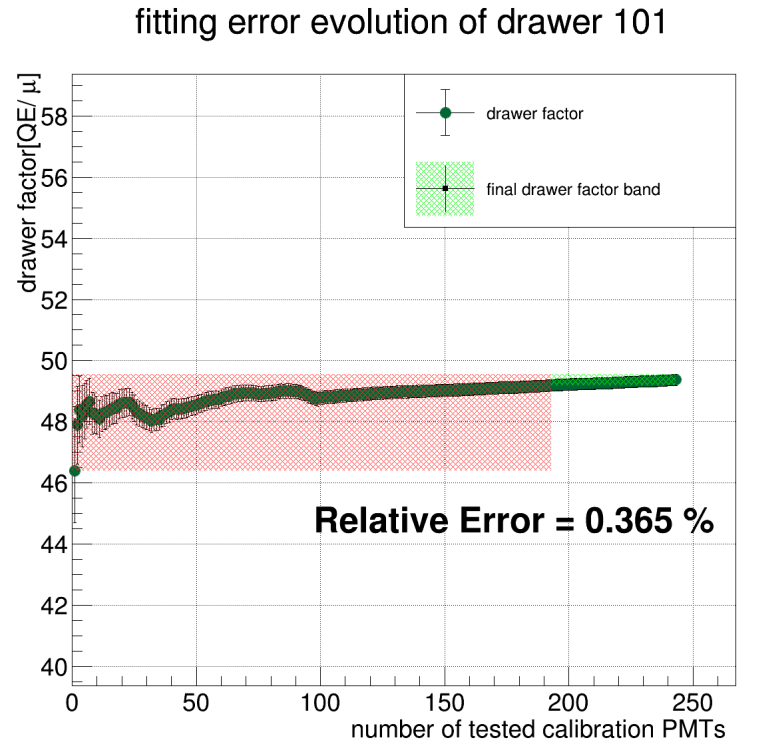
\includegraphics[width=\textwidth]{lt101} % 单图
%\end{figure}
%\end{column}
%\begin{column}{.45\textwidth}
%101抽屉一直放置参考PMT EA0419,抽屉因子$drawer_{factor}$拟合的结果随着时间漂移,这存在两种可能:
%\vspace{.5cm}
%\hrule{\textwidth}
%\vspace{.5cm}
signal waveform
\begin{itemize}
\item  $rise\ time=t_{.9rMaximum}-t_{.1rMaximum}$
\item $fall\ time=t_{.1fMaximum}-t_{.9fMaximum}$
\item $FWHM=t_{+1/2Maximum}-t_{-1/2Maximum}$
\end{itemize}

charge spectrum
\begin{itemize}
\item  $Gain=\frac{Q_{1pe}-Q_{0pe}}{Q_e}$
\item $PV=\frac{Peak_{spe}}{Valley_{spe}}$
\item $S/N=\frac{\sigma_{0pe}}{Q_{1pe}-Q_{0pe}}$
\item $Resolution=\frac{\sigma_{1pe}}{Q_{1pe}-Q_{0pe}}$
\end{itemize}


%\end{column}
%\end{columns}
\end{frame}
%%%%%%%%%%%%%%%%%%%%%%%%%%%%%%%%%%%%%%%%%%%%%%%%%%%%%%
\begin{frame}{calculation of $drawer_{factor}$}
\begin{figure}
\centering
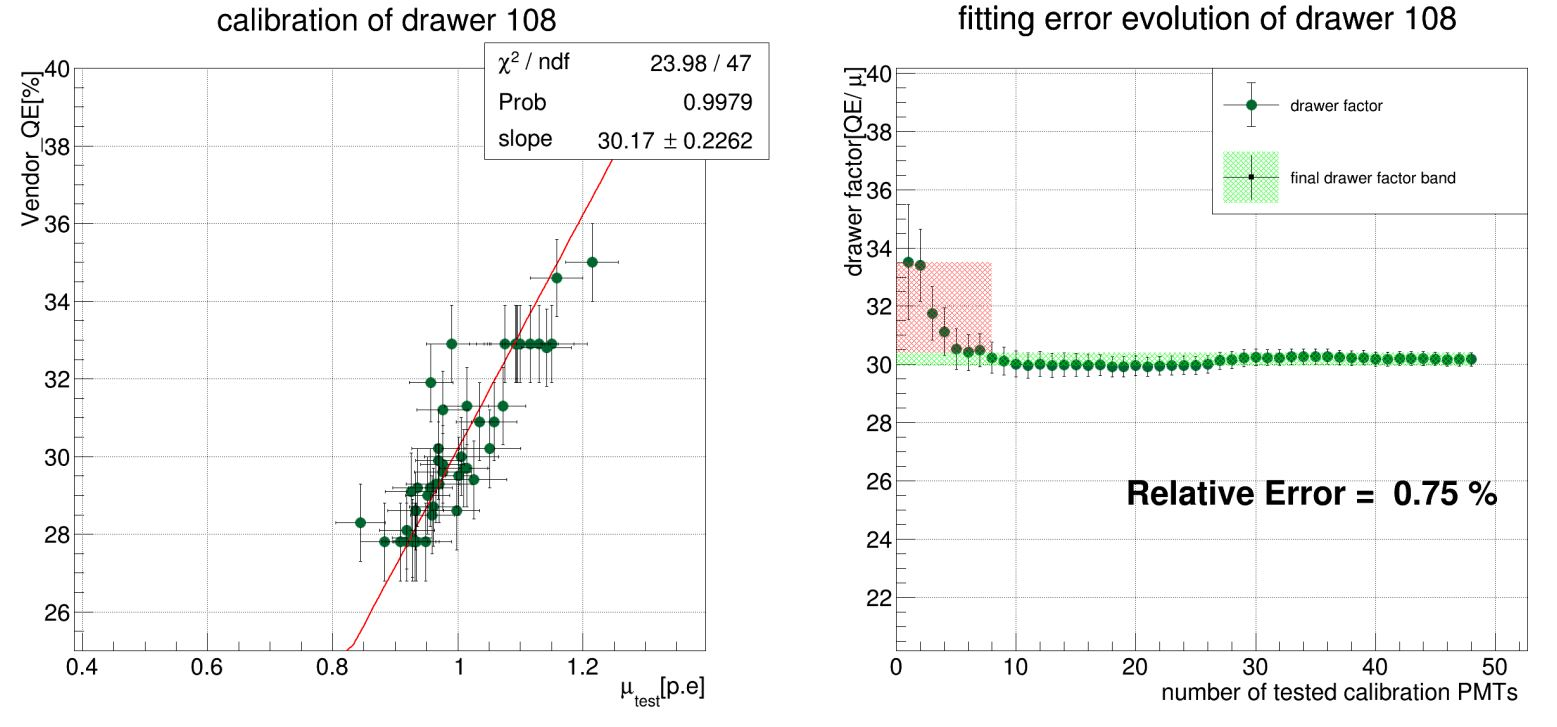
\includegraphics[width=\textwidth]{figures/mucal.JPG} % 单图
%\label{fig:wave2d}
\caption{fitting the drawer factor in one drawer}
\end{figure}
\end{frame}
\section{Statistical Sesults of Paramaters}
%%%%%%%%%%%%%%%%%%%%%%%%%%%%%%%%%%%%%%%%%%%
\begin{frame}{calculation of $PDE$}
we can obtain the average photon number $\mu_{test}$ from charge spectrum, along with the $drawer_{factor}$\footnote{Calibrate the drawer factor using PMT tested in the drawer which has vendor QE value.}, the PDE result from container system is:
\begin{equation}
PDE_{c}=\mu_{test}\times drawer_{factor}
\end{equation}
Then we map the PDE from container to the final PDE value with the help of container $f_{cs}$\footnote{linear correlation factor}:
\begin{equation}
PDE=PDE_{c}.f_{cs}+constant
\label{pde_formula}
\end{equation}
%根据公式\ref{pde_formula},通过$\mu_{test}$以及抽屉因子即可算出集装箱自己的PDE结果$PDE_c$。假设集装箱系统和扫描站对同一只PMT的测量结果是正比关系\footnote{参考王俊和王耀光的模拟结果},通过拟合线性参数$f_{cs}$可以算出最终的PDE。
\vspace{.5cm}
\hrule{\textwidth}
\vspace{.5cm}

\end{frame}
%%%%%%%%%%%%%%%%%%%%%%%%%%%%%%%%%%%%%%%%%%%
\begin{frame}{statistical results}
Mean value of parameters for HAMAMATSU-PMT and NNVT-PMT\footnote{For the parameter TTS, we need to test the internal time resolution firstly, since we found the TTS results is highly drawer related.}:

\vspace{.5cm}

\centering
\begin{tabular}{l|c|c}
\hline
\hline
parameters(mean)&  {\color{Blue} HAMAMATSU} & {\color{Blue}NNVT} \\\hline
DCR(kHz)&15.38&41.24\\
rise time(ns)&7.4& 3.2\\
fall time(ns)&10.36& 15.9\\
PV&3.39& 3.19\\
resolution&0.28& 0.35\\
HV@1E7(V)&1861& 1783\\
FWHM(ns)&9.08& 5.8\\
\hline
\end{tabular}
\end{frame}
%%%%%%%%%%%%%%%%%%%%%%%%%%%%%%%%%%%%%%%%%%%%%%%%%%%%%%
\begin{frame}{current PDE statistical results}
%amplitudes and  and charge intergrals of NNVT PMT is not as stable as HAMAMATSU PMT.
For NNVT PMT, the new version High-QE tubes have higher PDE with mean value about 30.5\%.
\begin{columns}
\begin{column}{.5\textwidth}
\begin{figure}
\centering
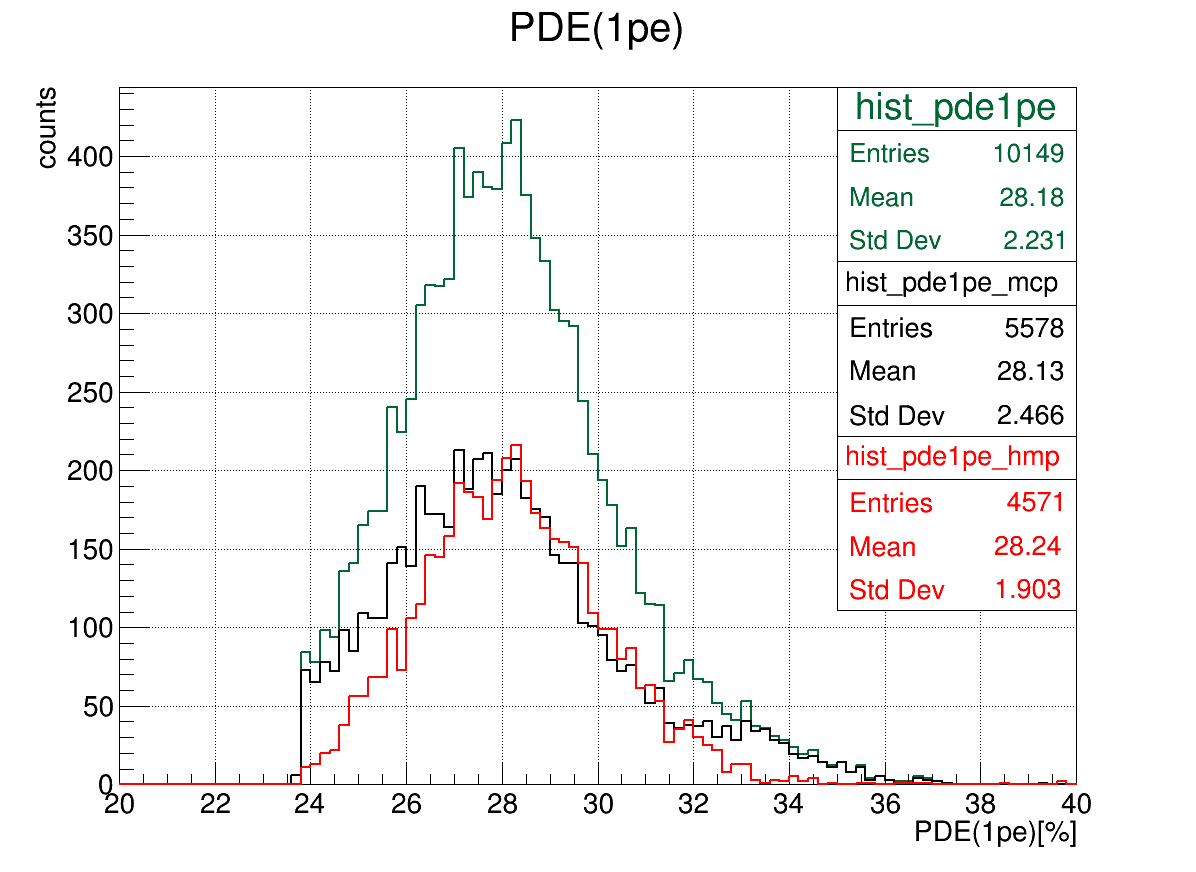
\includegraphics[width=\textwidth]{figures/pde1pe.png} % 单图
%\label{fig:wave2d}
\caption{PDE of tested PMT}
\end{figure}
\end{column}
\begin{column}{.5\textwidth}
\begin{figure}
\centering
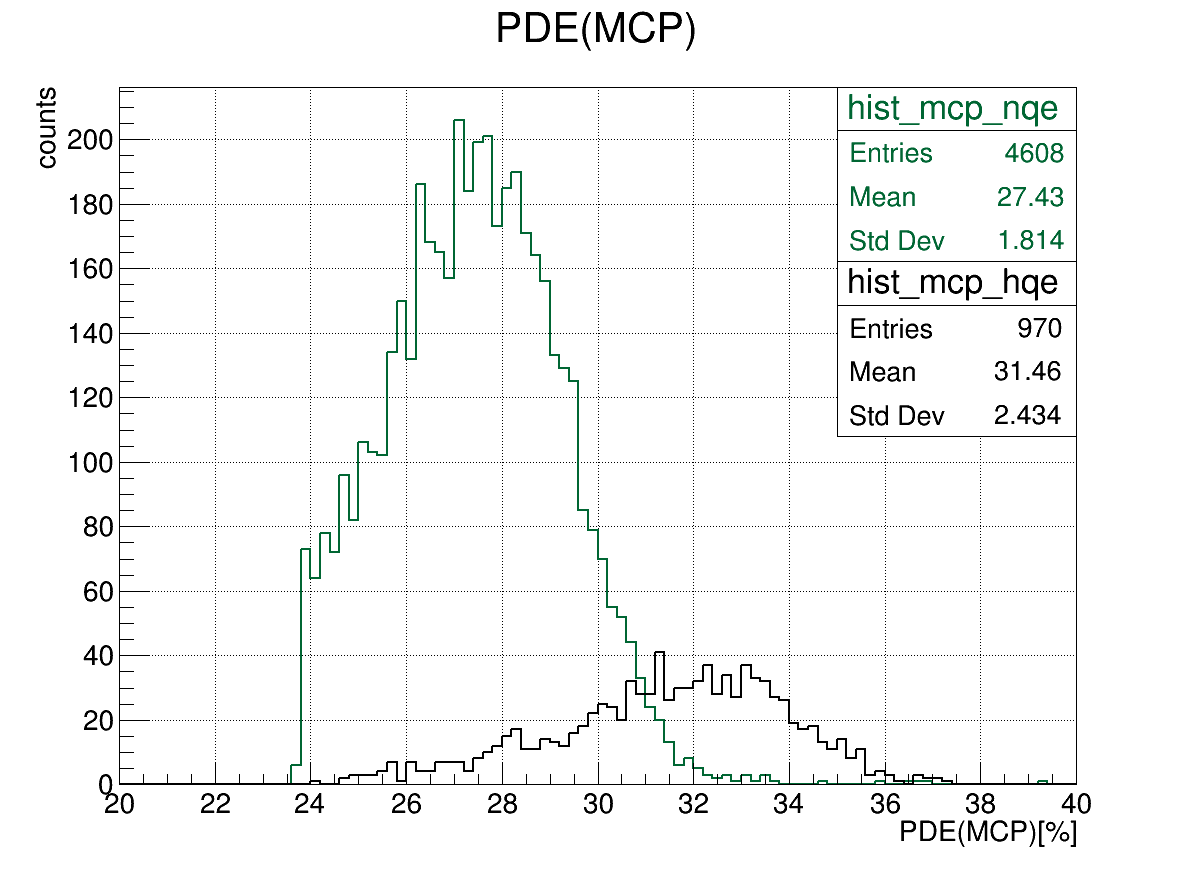
\includegraphics[width=\textwidth]{figures/pdemcp.png} % 单图
\caption{PDE of tested NNVT PMT}
\end{figure}
\end{column}
\end{columns}
\end{frame}
%%%%%%%%%%%%%%%%%%%%%%%%%%%%%%%%%%%%%%%%%%%%%%%%%%%%%%
\begin{frame}{predicted PDE statistical results}
%amplitudes and  and charge intergrals of NNVT PMT is not as stable as HAMAMATSU PMT.
CD will use $\sim$13k NNVT\footnote{with $\sim$11k high QE PMT and 2k low QE PMT} PMT, and 5k HAMAMATSU PMT, we can predict the final PDE and DCR distribution based on the current data:
\begin{columns}
\begin{column}{.5\textwidth}
\begin{figure}
\centering
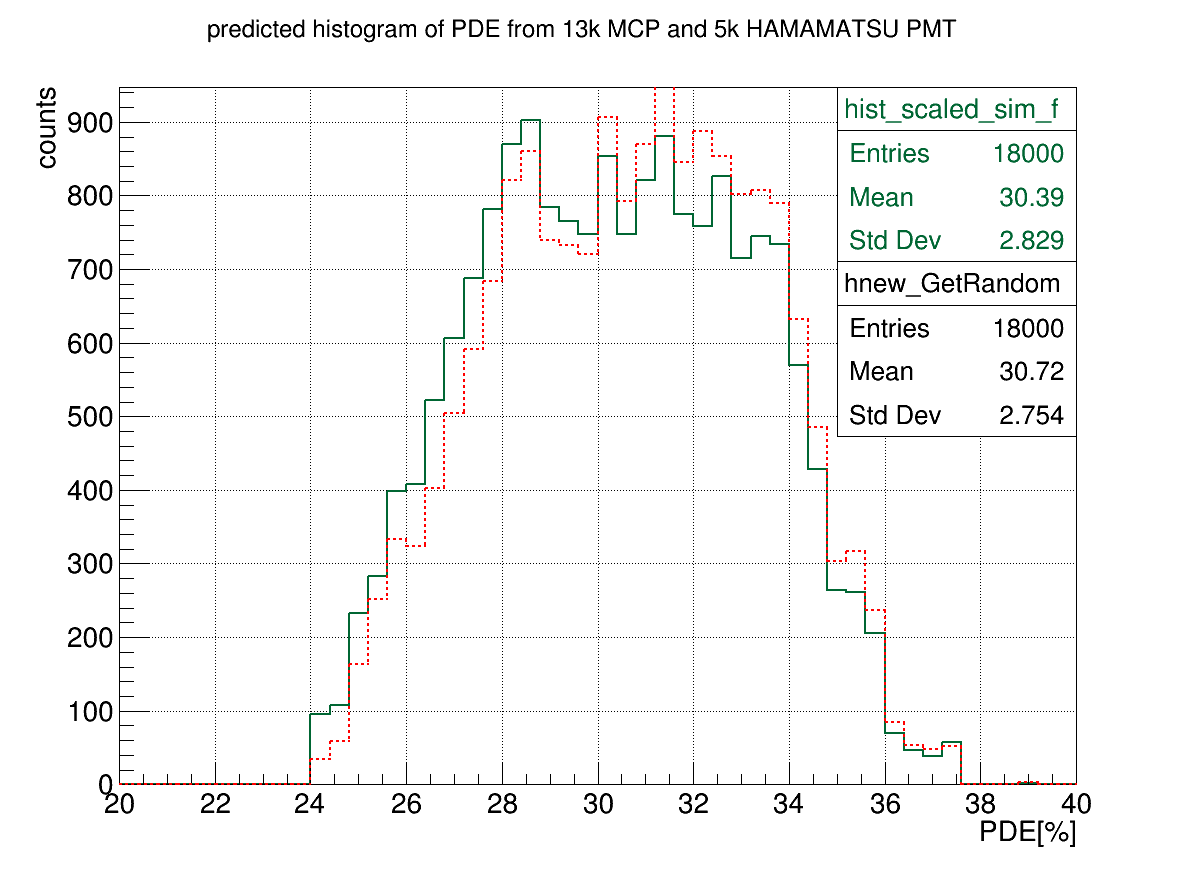
\includegraphics[width=\textwidth]{figures/sim.png} % 单图
%\label{fig:wave2d}
\caption{predicted PDE in CD}
\end{figure}
\end{column}
\begin{column}{.5\textwidth}
\begin{figure}
\centering
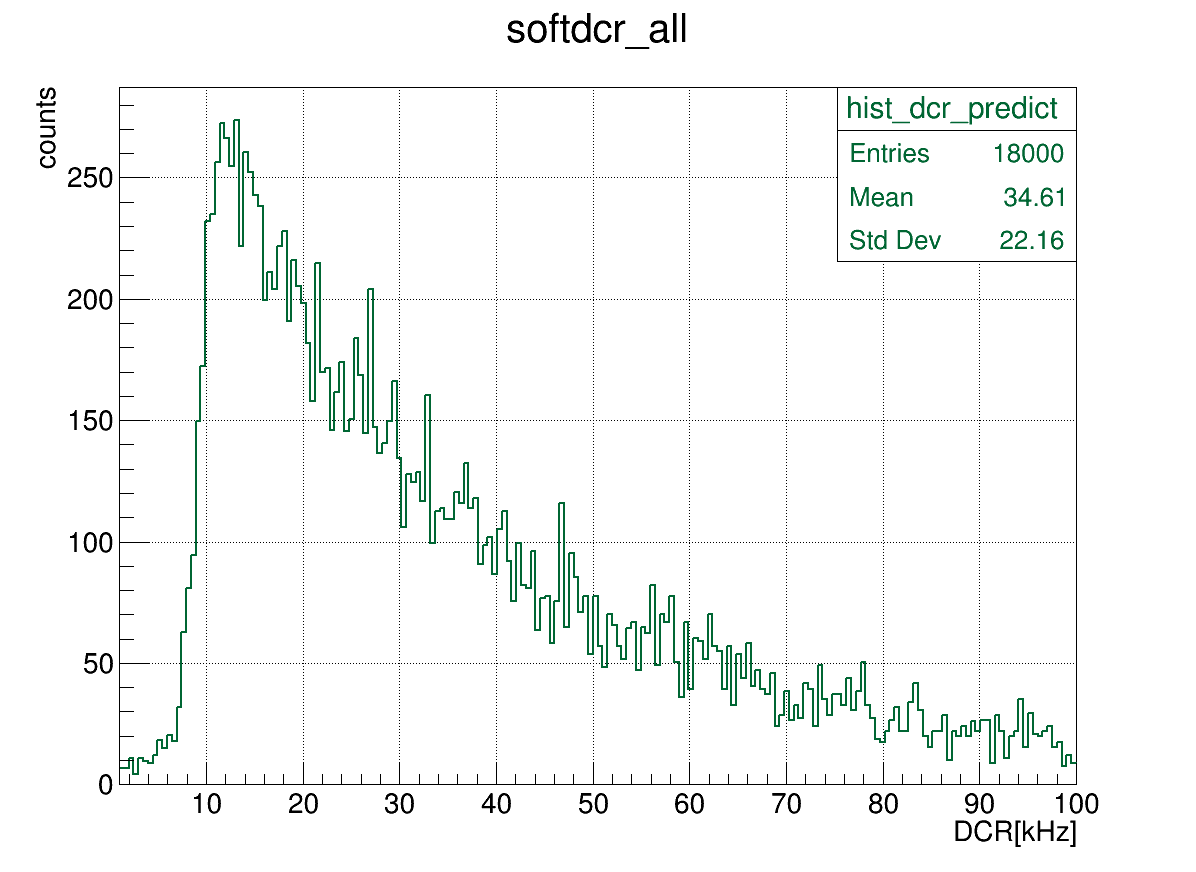
\includegraphics[width=\textwidth]{figures/dcr_p.png} % 单图
\caption{predicted DCR in CD}
\end{figure}
\end{column}
\end{columns}
\end{frame}
\section{Summary}

\begin{frame}{summary}
\begin{itemize}
\item  the charge and amplitude stability of HAMAMATSU PMT is better.
\item  $\sim$6k NNVT PMTs and 5k HAMAMATSU PMTs has been tested in container system, test results and test reports are avaliable from PMTDataBase\footnote{pmtdb.juno.ihep.ac.cn}.
\item we reject or accept one PMT according to its perfomance test results from container and scanning station.
\item  {\color{red}we need to study the "delay signal" of HAMAMATSU PMT and "big signal" of NNVT PMT\footnote{especially when PMT working in the multi-photon case}} in detail\footnote{one option is to transport several PMTs to SYSU for detailed study}.
\item the expected mean PDE value is 30.4\% and mean DCR value is $\sim$34kHz\footnote{will decrease after installation} in CD.
%\item 保存重要的测试信息和输出结果到PMT数据库,所有测试结果\footnote{包含集装测试历史数据}可以直接通过http://pmtdb.juno.ihep.ac.cn/\footnote{Query::LPMT Tested Reports} 查询得到
%\item 初步结论:目前现场5002支滨松PMT,382支外观检测不合格,5支HV不合格,2支波形较差,24支DCR不合格,9支PDE不合格。
\end{itemize}
\end{frame}

\begin{frame}
\centering {\zihao{0} \color{red} {THANKS}}
\end{frame}

\begin{frame}
\centering {\zihao{0} \color{red} {BACK-UP}}
\end{frame}

%\begin{table}[htbp]
%\caption{PMT typical performance}
%\resizebox{.8\textwidth}{!}{%
%\begin{tabular*}{.98\textwidth}{l|cccc}
%%\toprule
%\hline
%\hline
%Performance & PDE &DCR & TTS& uniformity \\
%\hline
%HAMAMATSU &  lower\% & 20 kHz& 3ns& worse \\
%NNVT  & higher\% & 40kHz & 7ns& better \\
%\hline
%\end{tabular*}
%%}
%\end{table}

%\end{frame}
%%%%%%%%%%%%%%%%%%%%%%%%%%%%%%%%%%%%%%%%%%%%%%%%%%%%%%
\begin{frame}{TTS of HAMAMATSU PMT}
\begin{figure}
\centering
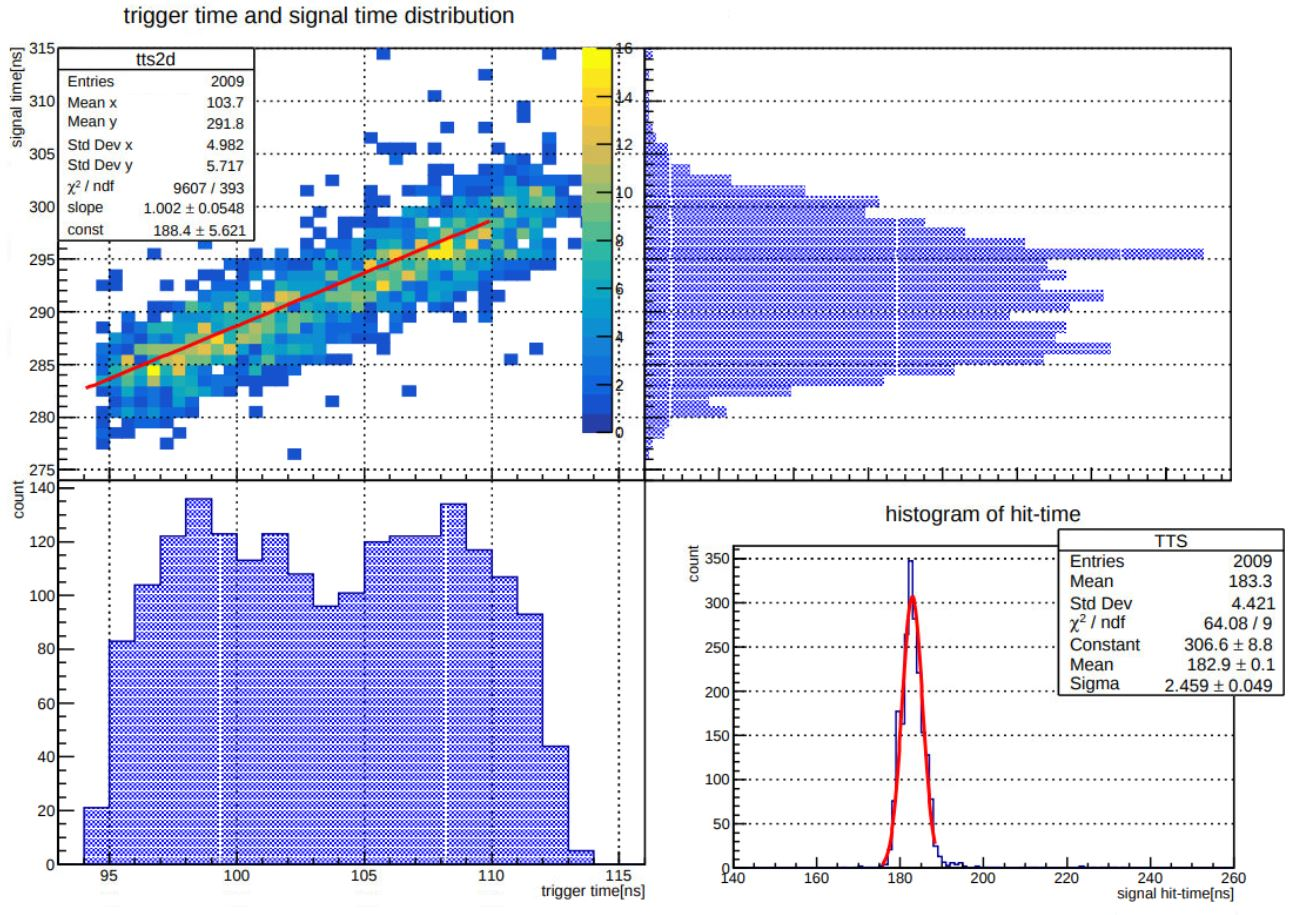
\includegraphics[width=.8\textwidth]{figures/hamtts.JPG} % 单图
%\label{fig:wave2d}
\caption{hittime and trigger time}
\end{figure}
\end{frame}
%%%%%%%%%%%%%%%%%%%%%%%%%%%%%%%%%%%%%%%%%%%%%%%%%%%%%%
\begin{frame}{TTS calculation of NNVT PMT}
\begin{figure}
\centering
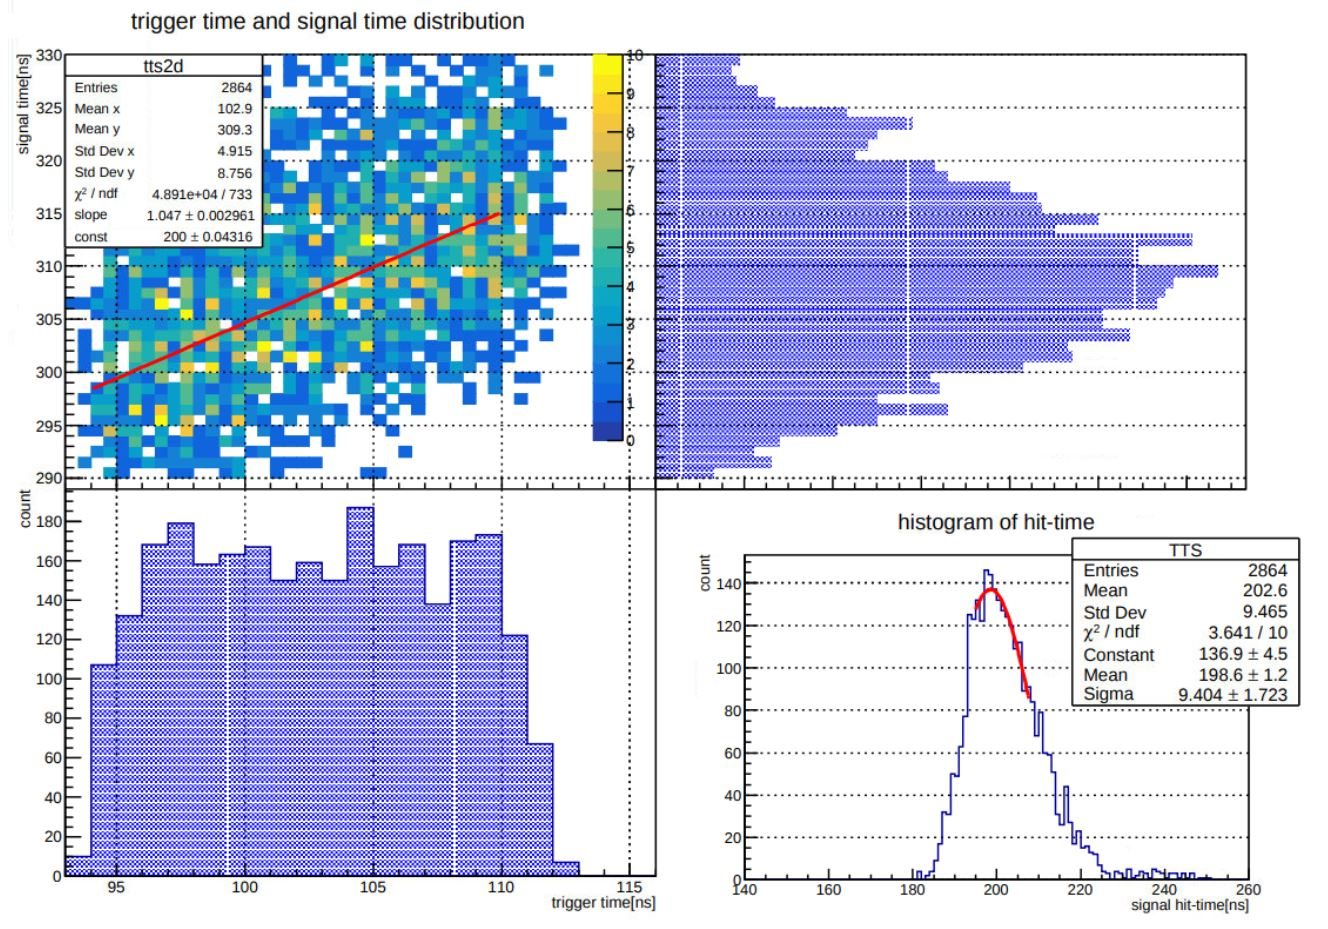
\includegraphics[width=.8\textwidth]{figures/mcptts.JPG} % 单图
%\label{fig:wave2d}
\caption{hittime and trigger time}
\end{figure}
\end{frame}
%%%%%%%%%%%%%%%%%%%%%%%%%%%%%%%%%%%%%%%%%%%
\begin{frame}{各个参数的统计结果-PDE}
\begin{figure}
\centering
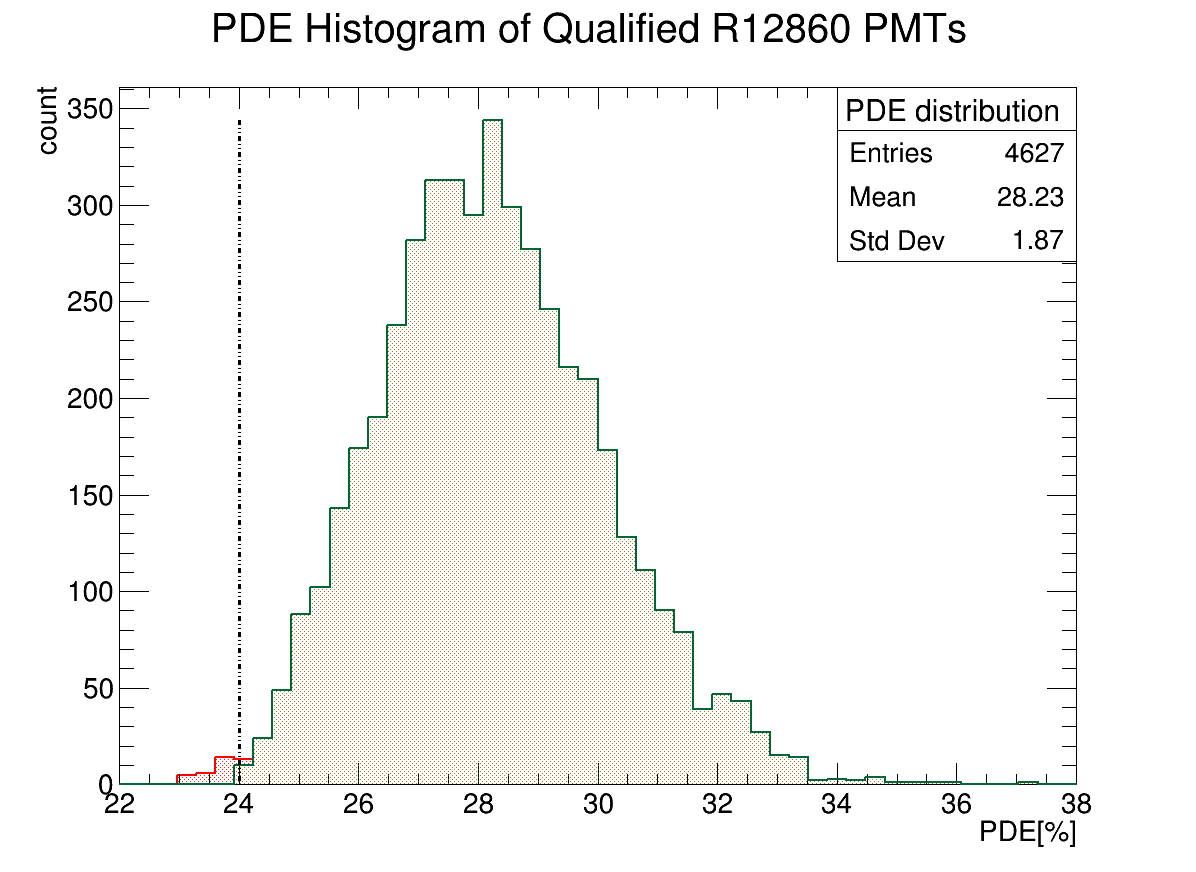
\includegraphics[width=0.78\textwidth]{figures/pde.png}
\end{figure}
\end{frame}
%%%%%%%%%%%%%%%%%%%%%%%%%%%%%%%%%%
\begin{frame}{PDE计算结果的初步对比}
对所有测试的PMT的PDE和测试现场的分析结果进行对比,发现存在少数PMT差别较大,需要进一步查找原因。
%\vspace{-.6cm}
\begin{columns}
\begin{column}{.5\textwidth}
\begin{figure}
\centering
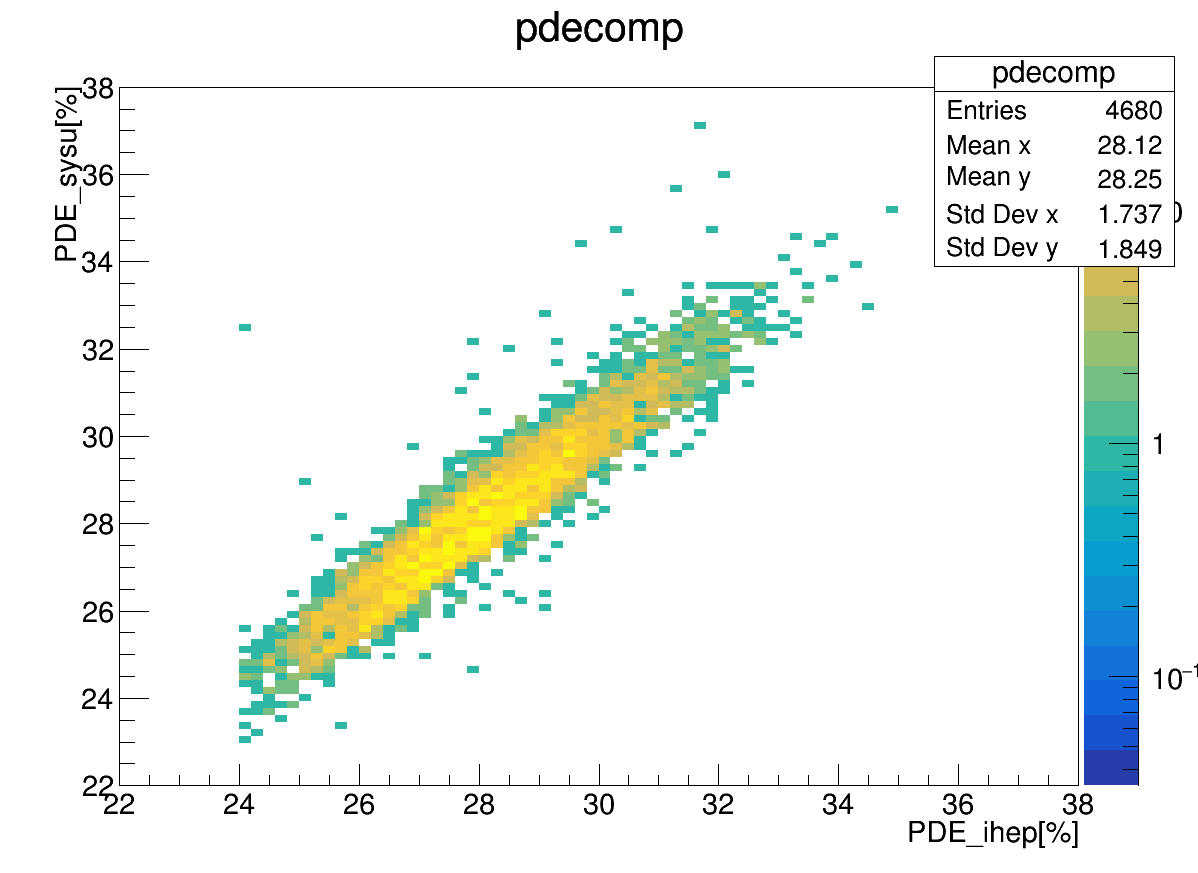
\includegraphics[width=\textwidth]{figures/pdecomparation.png} % 单图
%\label{fig:wave2d}
\caption{PDE结果的关联对比}
\end{figure}
\end{column}
\begin{column}{.5\textwidth}
\begin{figure}
\centering
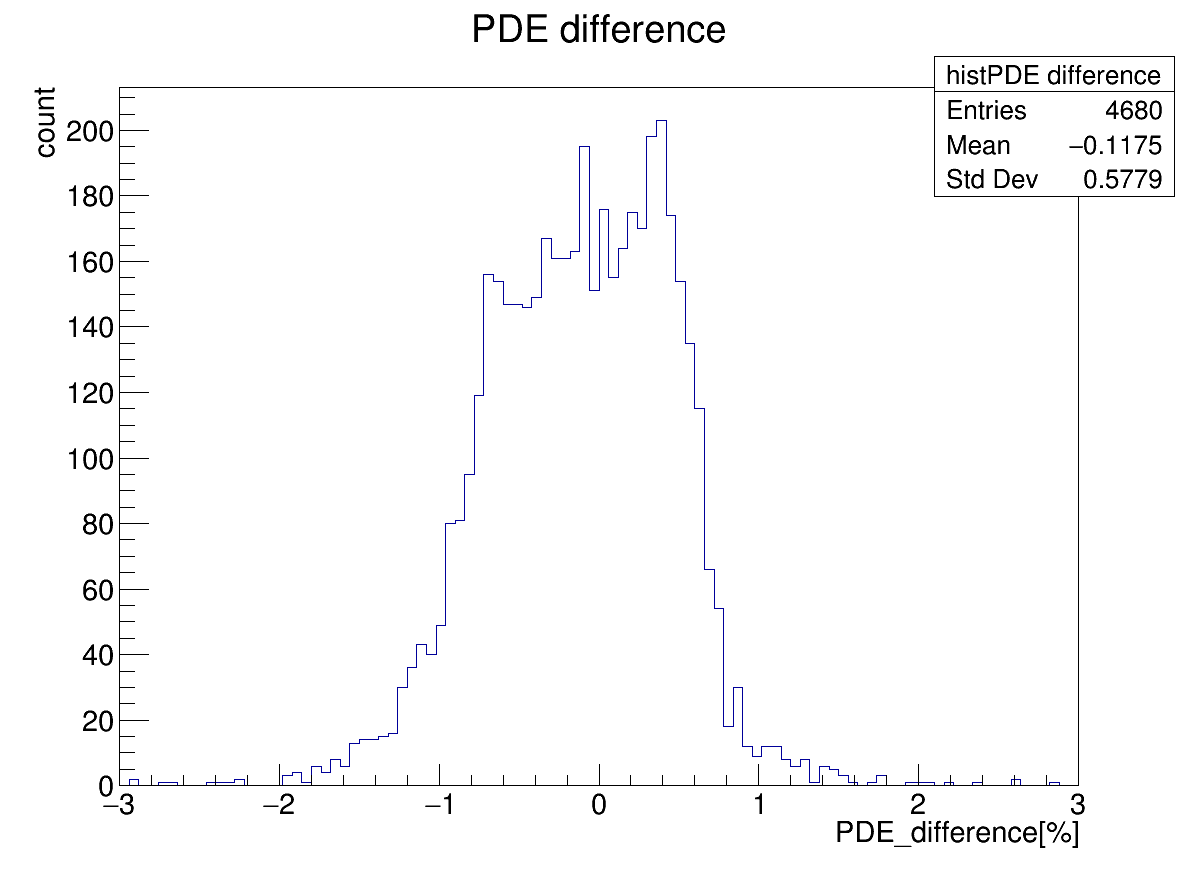
\includegraphics[width=\textwidth]{figures/pdedifference.png} % 单图
\caption{两种分析的差值分布}
\end{figure}
\end{column}
\end{columns}
\end{frame}
%%%%%%%%%%%%%%%%%%%%%%%%%%%%%%%%%%%%%%%%%%%
\begin{frame}{各个参数的统计结果-DCR}
\begin{figure}
\centering
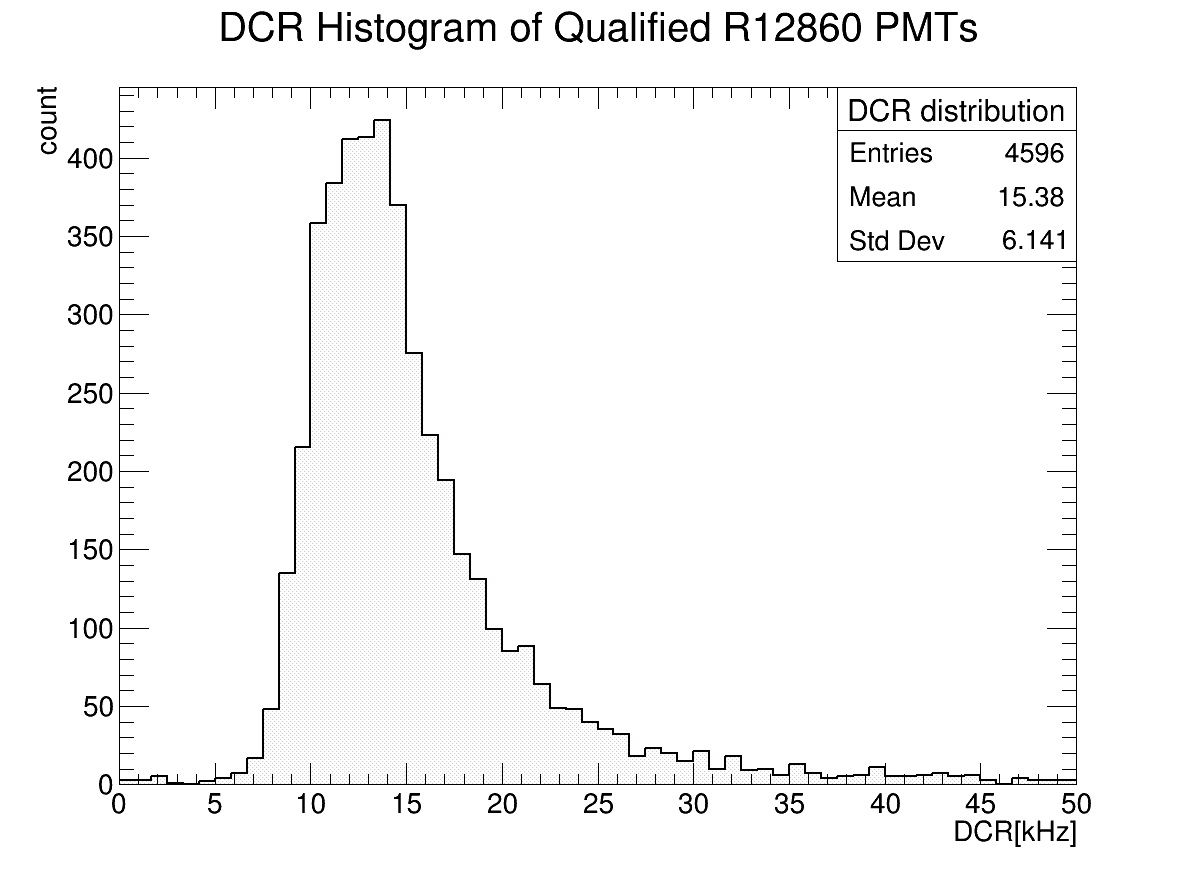
\includegraphics[width=0.78\textwidth]{figures/dcr.png}
\end{figure}
\end{frame}
%%%%%%%%%%%%%%%%%%%%%%%%%%%%%%%%%%%%%%%%%%%
\begin{frame}{各个参数的统计结果-Gain}
\begin{figure}
\centering
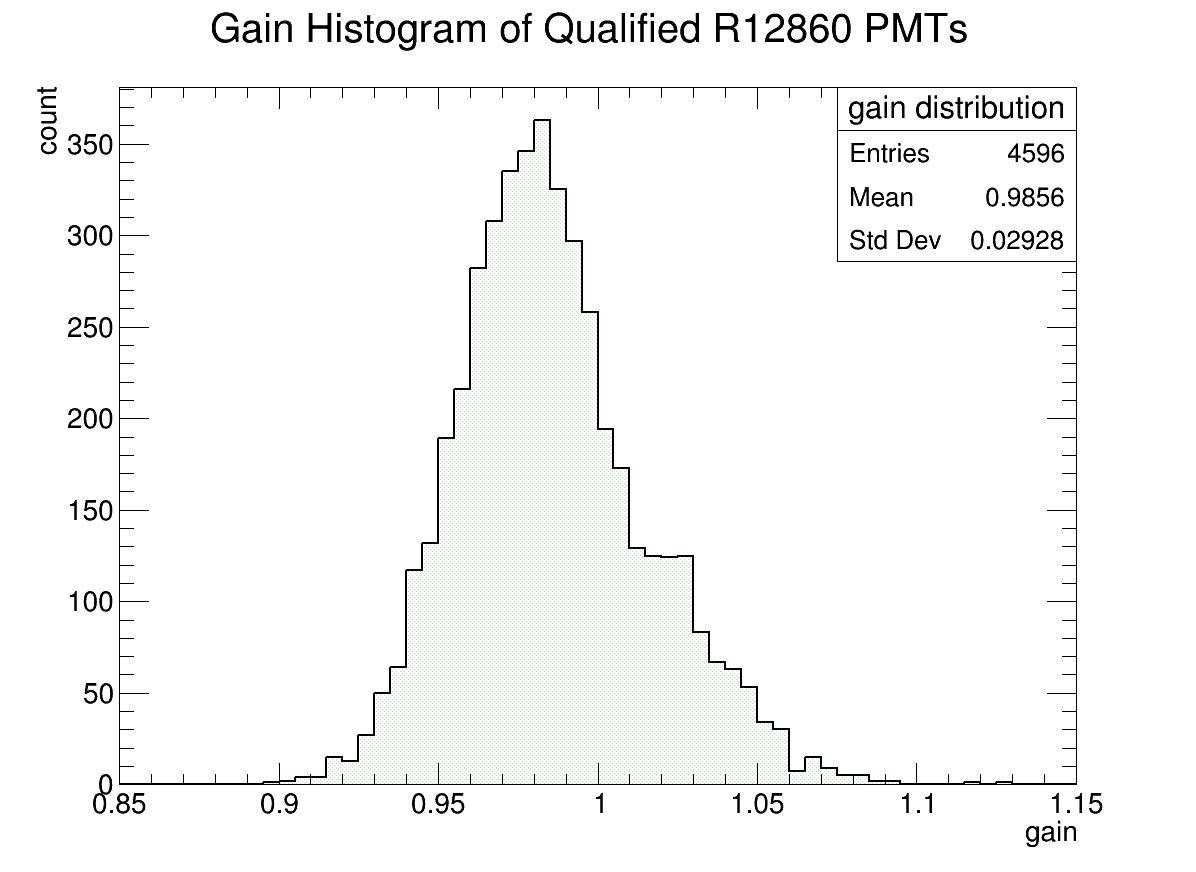
\includegraphics[width=0.78\textwidth]{figures/gain.png}
\end{figure}
\end{frame}
%%%%%%%%%%%%%%%%%%%%%%%%%%%%%%%%%%%%%%%%%%%
\begin{frame}{各个参数的统计结果-P/V}
\begin{figure}
\centering
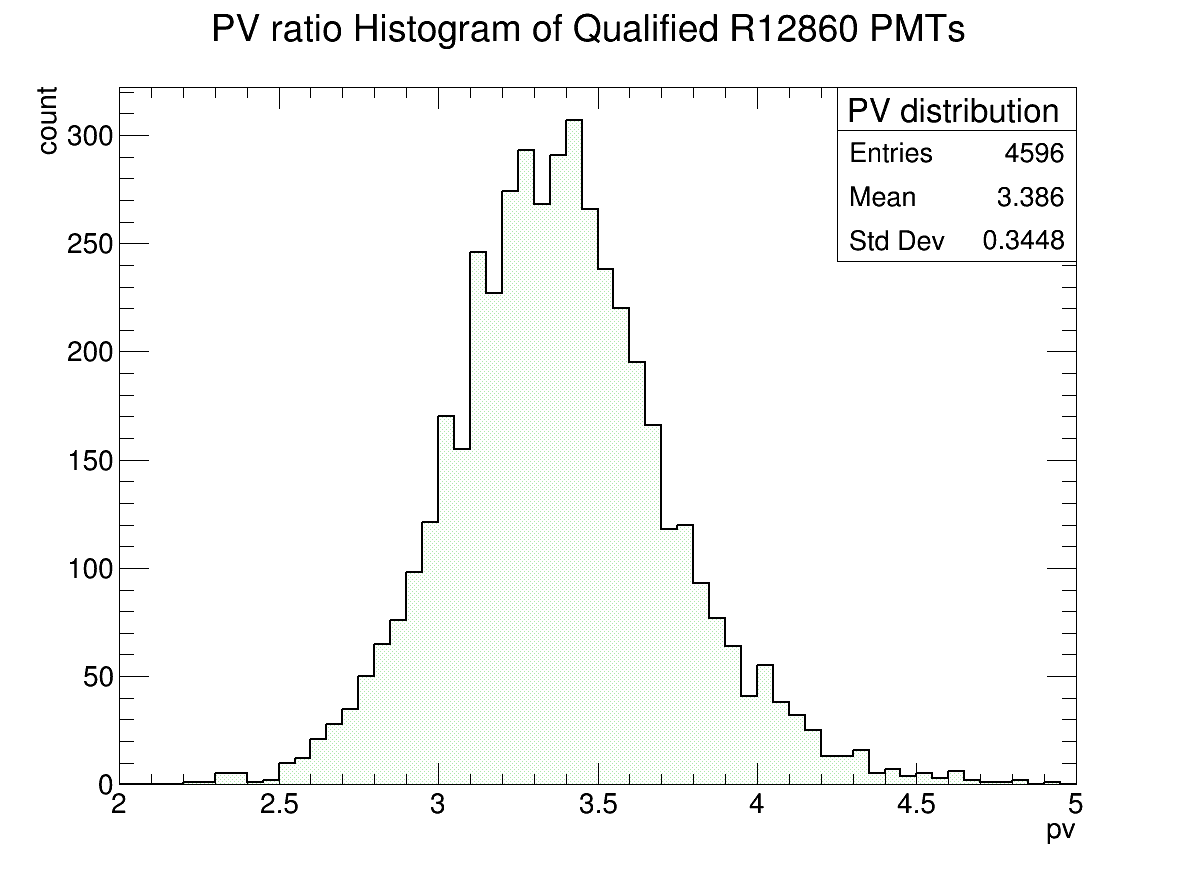
\includegraphics[width=0.78\textwidth]{figures/pv.png}
\end{figure}
\end{frame}
%%%%%%%%%%%%%%%%%%%%%%%%%%%%%%%%%%%%%%%%%%%
\begin{frame}{各个参数的统计结果-rise time}
\begin{figure}
\centering
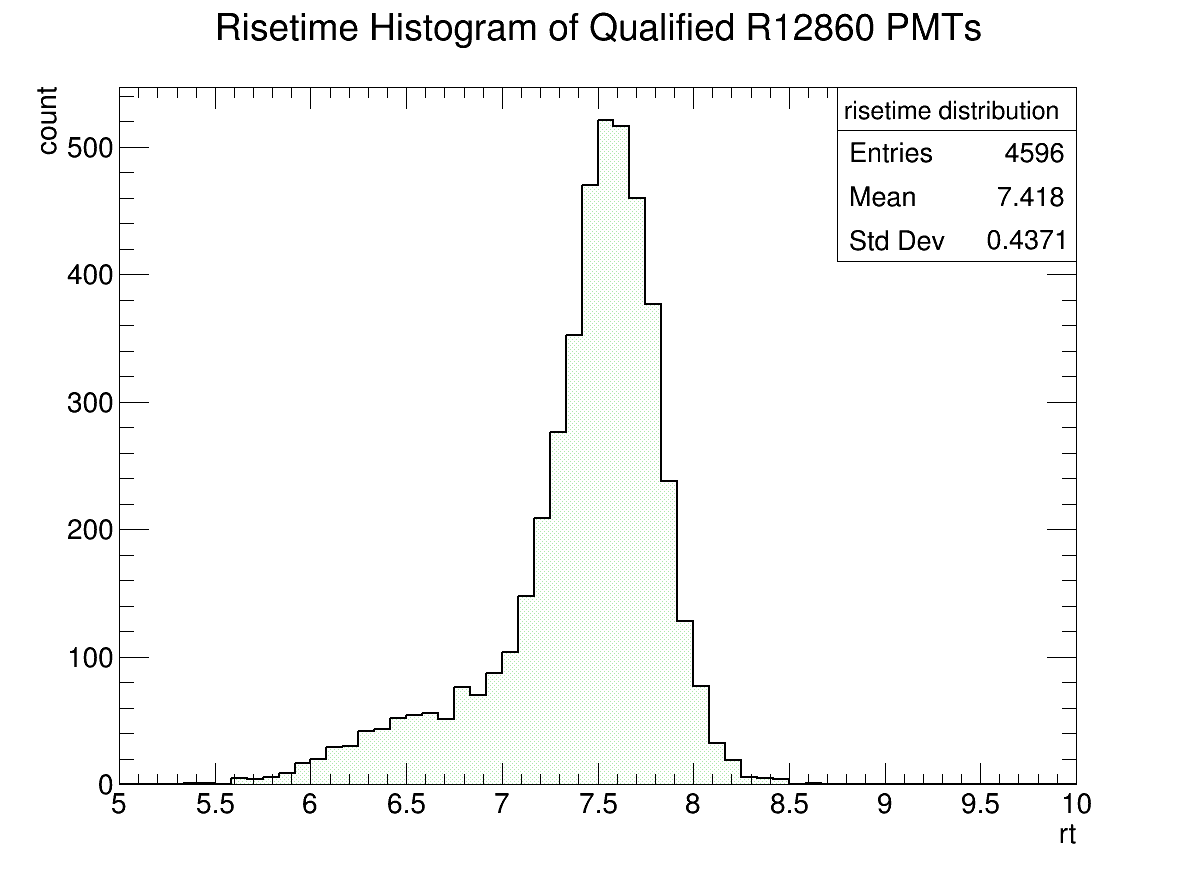
\includegraphics[width=0.78\textwidth]{figures/rt.png}
\end{figure}
\end{frame}
%%%%%%%%%%%%%%%%%%%%%%%%%%%%%%%%%%%%%%%%%%%
\begin{frame}{各个参数的统计结果-fall time}
\begin{figure}
\centering
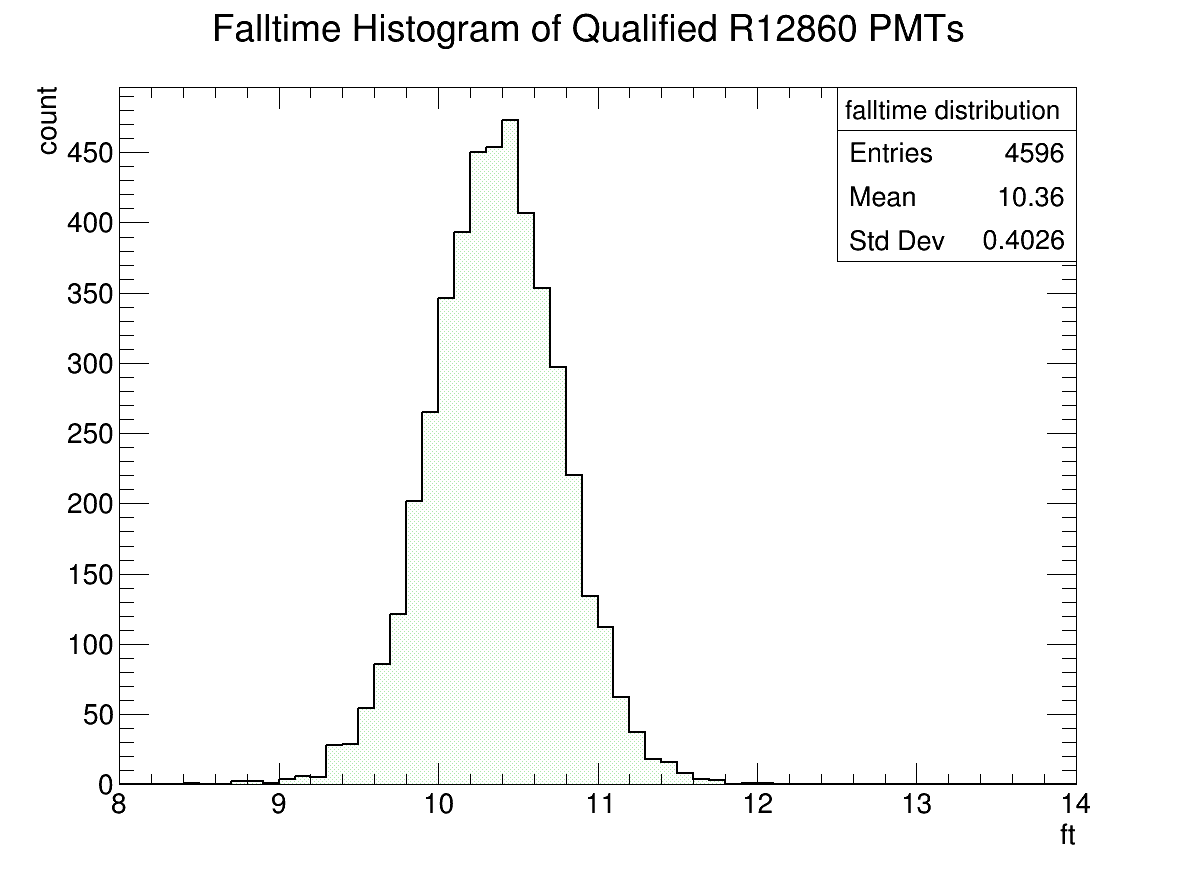
\includegraphics[width=0.78\textwidth]{figures/ft.png}
\end{figure}
\end{frame}
%%%%%%%%%%%%%%%%%%%%%%%%%%%%%%%%%%%%%%%%%%%
\begin{frame}{各个参数的统计结果-FWHM}
\begin{figure}
\centering
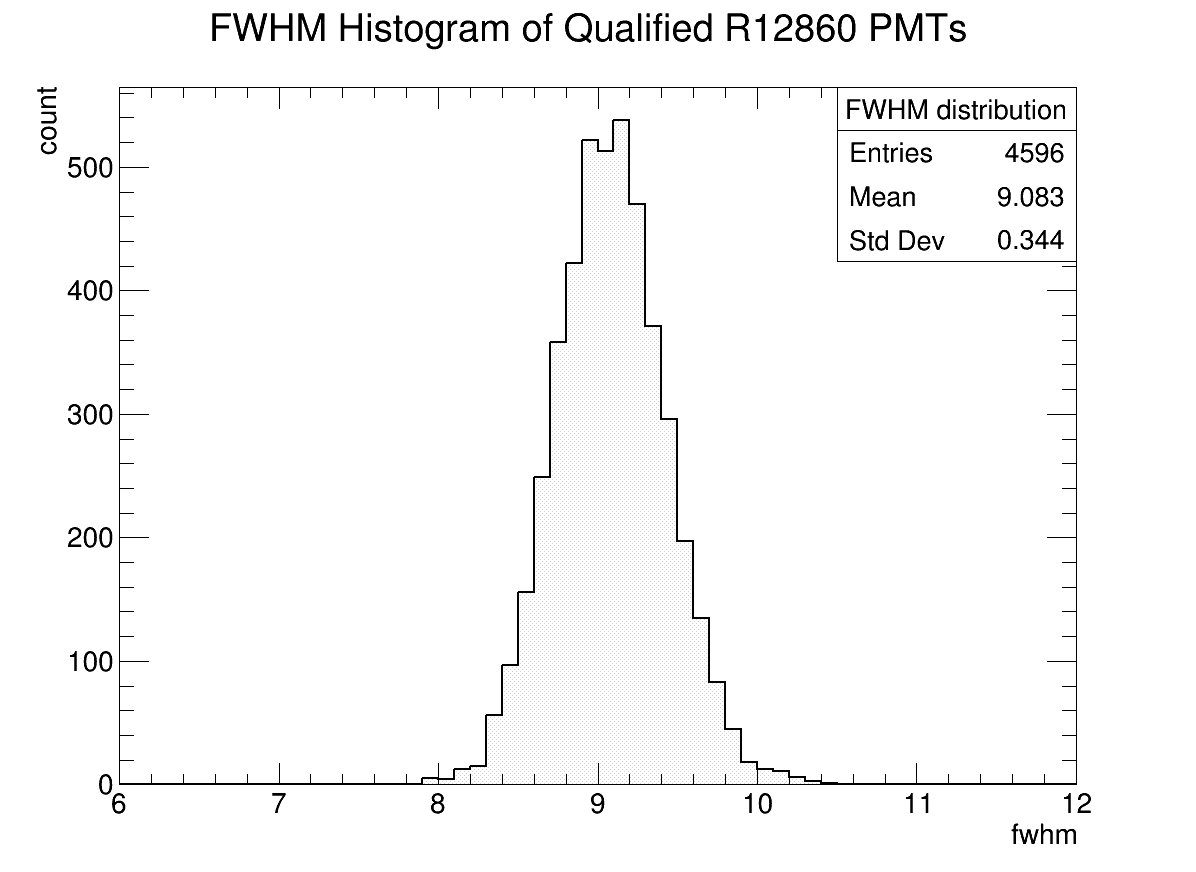
\includegraphics[width=0.78\textwidth]{figures/fwhm.png}
\end{figure}
\end{frame}
%%%%%%%%%%%%%%%%%%%%%%%%%%%%%%%%%%%%%%%%%%%
\begin{frame}{各个参数的统计结果-Resolution}
\begin{figure}
\centering
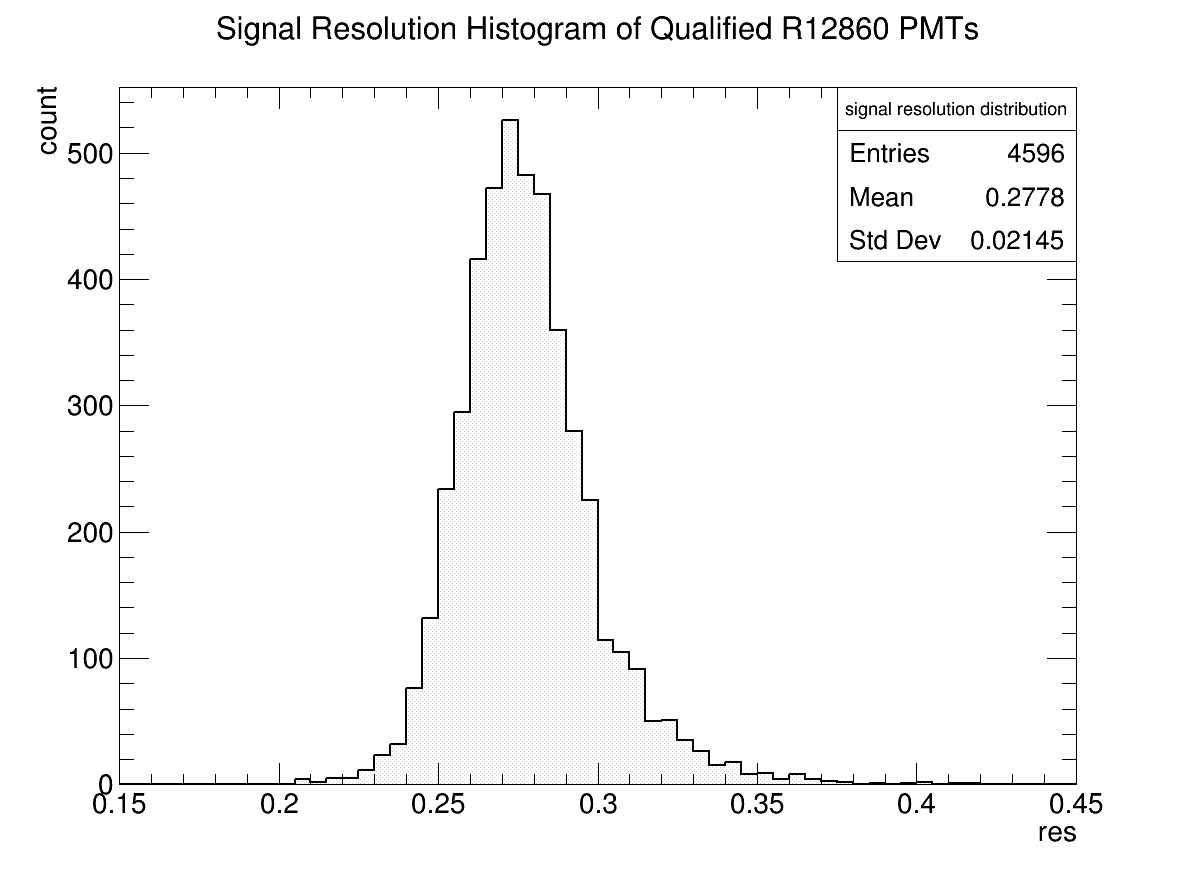
\includegraphics[width=0.78\textwidth]{figures/res.png}
\end{figure}
\end{frame}
%%%%%%%%%%%%%%%%%%%%%%%%%%%%%%%%%%%%%%%%%%%
\begin{frame}{各个参数的统计结果-S/N}
\begin{figure}
\centering
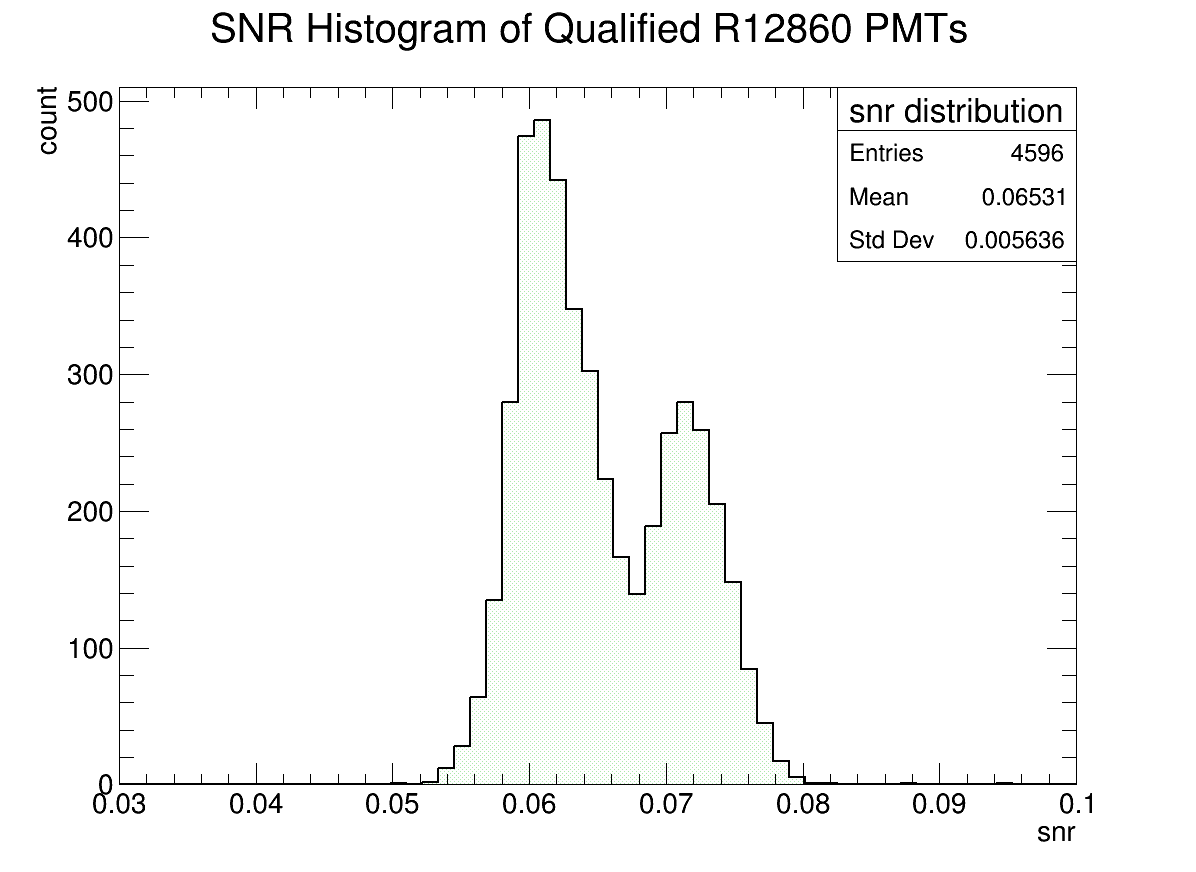
\includegraphics[width=0.78\textwidth]{figures/snr.png}
\end{figure}
\end{frame}
%%%%%%%%%%%%%%%%%%%%%%%%%%%%%%%%%%%%%%%%%%%
\begin{frame}{各个参数的统计结果-HV}
\begin{figure}
\centering
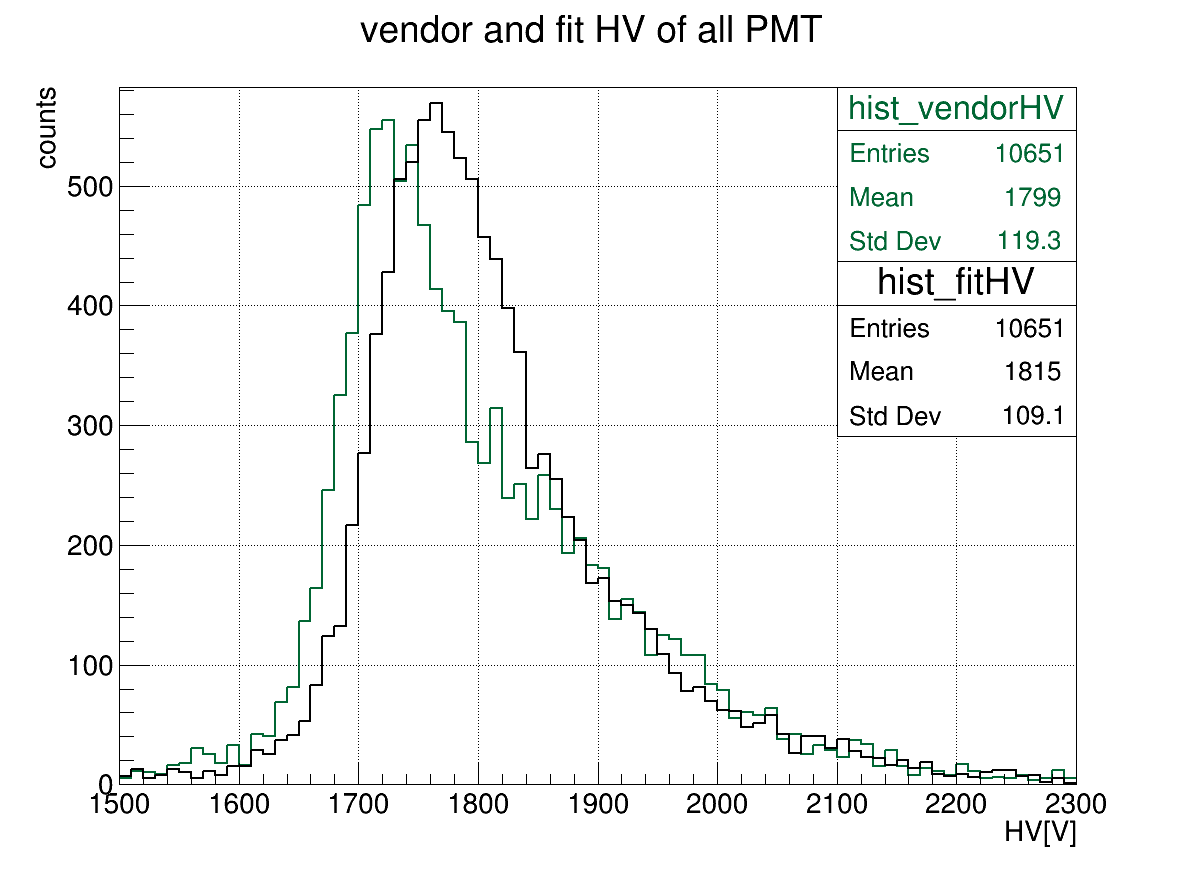
\includegraphics[width=0.78\textwidth]{figures/vendorHV.png}
\end{figure}
\end{frame}
%%%%%%%%%%%%%%%%%%%%%%%%%%%%%%%%%%%%%%%%%%%%
%\begin{frame}{测试结果的输出}
%在完成每一只PMT的数据分析之后,输出重要的信息和数据:
%\begin{itemize}
%\item 测试信息:测试时间、集装箱编号、抽屉编号 、mass number等
%\item 性能测试信息:各种波形图、参数计算的中间histogram
%\item 各个参数的计算结果、拟合信息
%\item 集装箱测试的历史记录、扫描站的测试结果
%\item 最终合格与否的结论标签
%\end{itemize}
%\vspace{.5cm}
%\hrule{\textwidth}
%\vspace{.5cm}
%\alert{对于每一只PMT,结合集装箱的多次测量结果以及扫描站复测结果,确保给出正确的最终结论。}
%\end{frame}
%%%%%%%%%%%%%%%%%%%%%%%%%%%%%%%%%%%%%%%%%%%%
%\begin{frame}{测试结果报告-reject}
%\begin{figure}
%\centering
%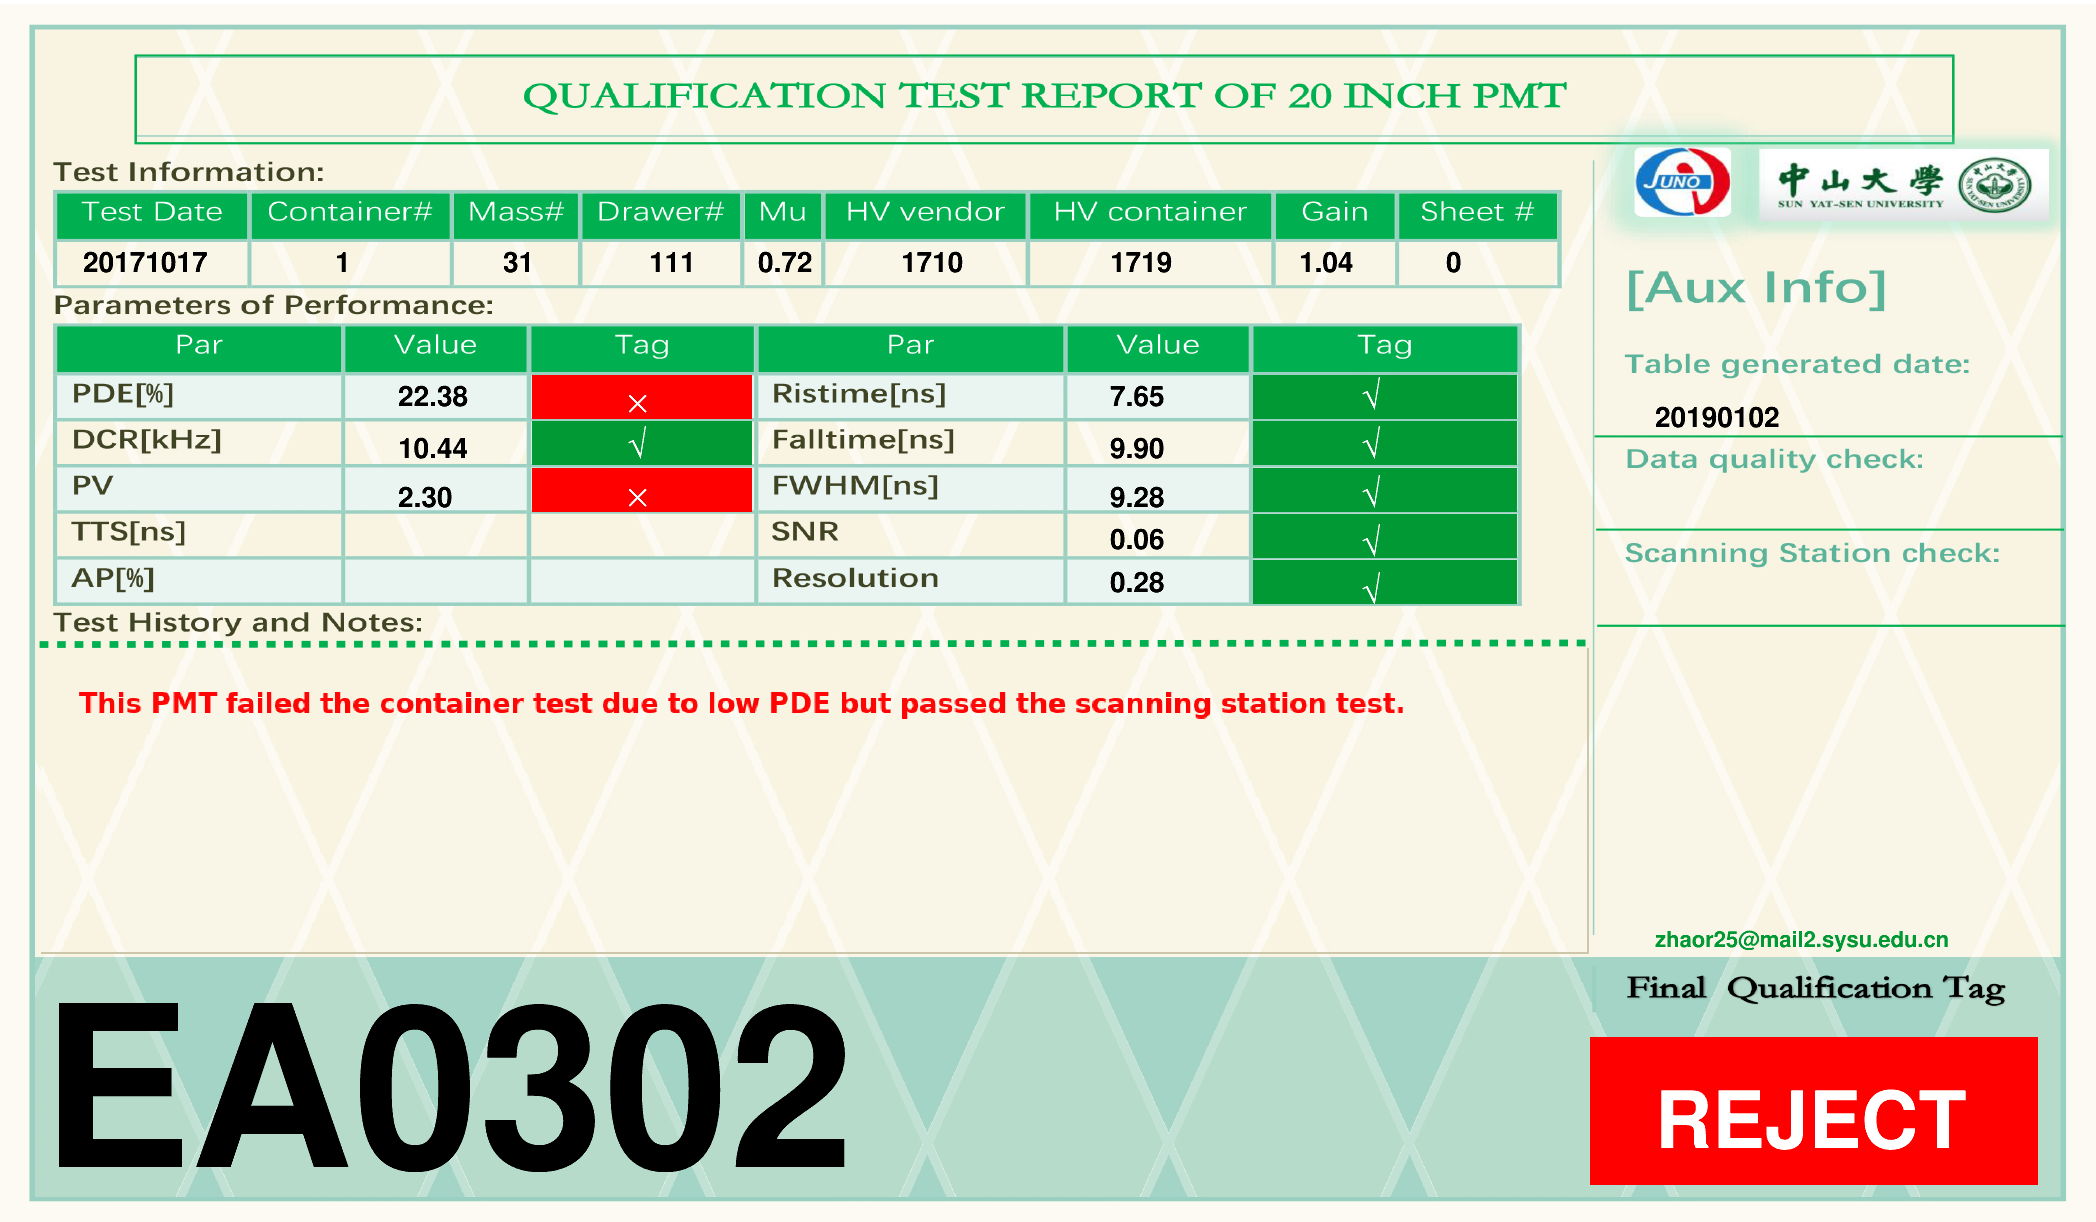
\includegraphics[width=1.0\textwidth]{figures/SN_EA0302_pde0_dcr1_HV1_pv0_rt1_tag0.png}
%\end{figure}
%\end{frame}
%
%%%%%%%%%%%%%%%%%%%%%%%%%%%%%%%%%%%%%%%%%%%%%%%%%%%%%%%%%%%%%%%%%%%%
%%%%%%%%%%%%%%%%%%%%%%%%%%%%%%%%%%%%%%%%%%%%%%%%%%%%%%%%%%%%%%%%%%%%
%\begin{frame}{PDE计算结果}
%将MCP-PMT的高量子效率分开处理,统计集装箱1测量到的MCP-PMT的PDE结果\footnote{更新到2018-10-17的测试结果}:
%%\hrule{\textwidth}
%\begin{columns}
%\begin{column}{.56\textwidth}
%\begin{figure}
%\centering
%\includegraphics[width=\textwidth]{mcppde}
%\end{figure}
%\end{column}
%\begin{column}{.4\textwidth}
%\alert{MCP的高量子效率版本PDE相对增加了15.8\%}
%\vspace{.5cm}
%\hrule{\textwidth}
%\vspace{.5cm}
%PDE 的统计结果和现场算法得到的结果一致。\\
%MCP:27.5\leftrightarrow \alert{27.55}\\
%HAMAMATSU:28.5\leftrightarrow \alert{28.56}
%\end{column}
%%\end{figure}
%\end{columns}
%\end{frame}
%%%%%%%%%%%%%%%%%%%%%%%%%%%%%%%%%%%%%%%%%%%%%%%%%%%%%%%%%%%%%%%
%%%%%%%%%%%%%%%%%%%%%%%%%%%%%%%%%%%%%%%%%%%%%%%%%%%%%%%%%%%%%%%

%\begin{frame}[allowframebreaks]
%\frametitle{References}
%\scriptsize
%\bibliographystyle{authordate1}
%\bibliography{R-GLMM-pkgs}
%\end{frame}

\appendix

\section*{附录}

%\begin{frame}{其他重要参数的check}
%MCP-PMT的参数对比:
%
%\vspace{.5cm}
%
%\centering
%\begin{tabular}{l|c|c}
%\hline
%\hline
%参数(平均值)&  {\color{Blue} 我的结果} & {\color{Blue}测试现场结果} \\\hline
%暗计数(kHz)&41.4&44.3\\
%信号上升时间(ns)&3.2& 4.6\\
%信号下降时间(ns)&15.9& 16.2\\
%峰谷比&3.19& 4.4\\
%分辨率&0.35& 0.32\\
%高压(V)&1783& 1784\\
%信号半高宽(ns)&5.8& 7.7\\
%\hline
%\end{tabular}
%\end{frame}
%\begin{frame}{drawer-calibration}
%\vspace{-.5cm}
%\includegraphics[width=0.45\textwidth]{sta101-0}
%\includegraphics[width=0.45\textwidth]{sta101-1}
%\includegraphics[width=0.45\textwidth]{sta101-2}
%\includegraphics[width=0.45\textwidth]{sta101-3}
%\includegraphics[width=0.45\textwidth]{sta101-4}
%\includegraphics[width=0.45\textwidth]{sta101-5}
%\end{frame}
%\begin{frame}{drawer-calibration}
%\vspace{-.5cm}
%\includegraphics[width=0.45\textwidth]{sta101-6}
%\includegraphics[width=0.45\textwidth]{sta101-7}
%\includegraphics[width=0.45\textwidth]{sta101-8}
%\includegraphics[width=0.45\textwidth]{sta101-9}
%\includegraphics[width=0.45\textwidth]{sta101-10}
%\includegraphics[width=0.45\textwidth]{sta101-11}
%\end{frame}
%\begin{frame}{drawer-calibration}
%\vspace{-.5cm}
%\includegraphics[width=0.45\textwidth]{sta101-12}
%\includegraphics[width=0.45\textwidth]{sta101-13}
%\includegraphics[width=0.45\textwidth]{sta101-14}
%\includegraphics[width=0.45\textwidth]{sta101-15}
%\includegraphics[width=0.45\textwidth]{sta101-16}
%\includegraphics[width=0.45\textwidth]{sta101-17}
%\end{frame}
%\begin{frame}{drawer-calibration}
%\vspace{-.5cm}
%\includegraphics[width=0.45\textwidth]{sta101-18}
%\includegraphics[width=0.45\textwidth]{sta101-19}
%\includegraphics[width=0.45\textwidth]{sta101-20}
%\includegraphics[width=0.45\textwidth]{sta101-21}
%\includegraphics[width=0.45\textwidth]{sta101-22}
%\includegraphics[width=0.45\textwidth]{sta101-23}
%\end{frame}
%\begin{frame}{drawer-calibration}
%\vspace{-.5cm}
%\includegraphics[width=0.45\textwidth]{sta101-24}
%\includegraphics[width=0.45\textwidth]{sta101-25}
%\includegraphics[width=0.45\textwidth]{sta101-26}
%\includegraphics[width=0.45\textwidth]{sta101-27}
%\includegraphics[width=0.45\textwidth]{sta101-28}
%\includegraphics[width=0.45\textwidth]{sta101-29}
%\end{frame}
%\begin{frame}{drawer-calibration}
%\vspace{-.5cm}
%\includegraphics[width=0.45\textwidth]{sta101-30}
%\includegraphics[width=0.45\textwidth]{sta101-31}
%\includegraphics[width=0.45\textwidth]{sta101-32}
%\includegraphics[width=0.45\textwidth]{sta101-33}
%\includegraphics[width=0.45\textwidth]{sta101-34}
%\end{frame}
%%%%%%%%%%%%%%%%%%%%%%%%%%%%%%%%%%%%%%%%%
\begin{frame}{抽屉因子的比较}
factor\_1是我的结果,factor\_2是张海琼的结果。$y=1.148x+0.998$
\vspace{-.05cm}
\begin{figure}
\includegraphics[width=0.72\textwidth]{drawerfactors}
\caption{抽屉因子和现场使用值的对比}
\end{figure}
\end{frame}

%\begin{frame}{两套装置测量结果的转换}
%利用$PDE_c$和$PDE_s$对所有高量子效率MCP-PMT拟合$f_{cs}$的结果:
%\begin{figure}
%\centering
%\includegraphics[width=0.68\textwidth]{fit_mcp_hqe_noint}
%\end{figure}
%\end{frame}
%\begin{frame}{两套装置测量结果的转换}
%利用$PDE_c$和$PDE_s$对所有低量子效率MCP-PMT拟合$f_{cs}$的结果:
%\begin{figure}
%\centering
%\includegraphics[width=0.68\textwidth]{fit_mcp_nqe_noint}
%\end{figure}
%\end{frame}
%%%%%%%%%%%%%%%%%%%%%%%%%%%%%%%%%%%%%%%%%%%
\begin{frame}{参考管稳定性}
\begin{figure}
\centering
\includegraphics[width=0.68\textwidth]{ref_sta}
\end{figure}
\end{frame}
%%%%%%%%%%%%%%%%%%%%%%%%%%%%%%%%%%%%%%%%%%%
\begin{frame}{参考管电压稳定性}
新DAQ对系统的性能产生了影响,高压平均值发生了变化:
\begin{figure}
\centering
\includegraphics[width=0.68\textwidth]{ref_HV_sta}
\end{figure}
\end{frame}
%%%%%%%%%%%%%%%%%%%%%%%%%%%%%%%%%%%%%%%%%%%
%\begin{frame}{EA0419}
%参考管EA0419一直在101抽屉,它的测量结果反映了集装箱测试系统的性能和稳定性:
%\begin{figure}
%\centering
%\includegraphics[width=0.98\textwidth]{101_sta}
%\end{figure}
%\end{frame}
%%%%%%%%%%%%%%%%%%%%%%%%%%%%%%%%%%%%%%%%%%%
\begin{frame}{暗计数}
\begin{figure}
\centering
\includegraphics[width=0.48\textwidth]{vendordcr_mcp}
\includegraphics[width=0.48\textwidth]{vendordcr_hmp}
\end{figure}
\end{frame}
%%%%%%%%%%%%%%%%%%%%%%%%%%%%%%%%%%%%%%%%%%%
\begin{frame}{上升时间和下降时间分布}
\begin{figure}
\centering
\includegraphics[width=0.48\textwidth]{risetime}
\includegraphics[width=0.48\textwidth]{falltime}
\end{figure}
\end{frame}
%%%%%%%%%%%%%%%%%%%%%%%%%%%%%%%%%%%%%%%%%%%
